\documentclass[10pt]{article}
\usepackage{times}
\usepackage{geometry}
\usepackage{listings}
\usepackage{color}
\usepackage{xcolor}
\usepackage[most]{tcolorbox}
\definecolor{bg}{RGB}{240,248,255}
 
\definecolor{codegreen}{rgb}{0,0.6,0}
\definecolor{codegray}{rgb}{0.5,0.5,0.5}
\definecolor{codepurple}{rgb}{0.58,0,0.82}
\definecolor{backcolour}{rgb}{0.95,0.95,0.92}
\renewcommand{\baselinestretch}{1.4} 

\lstdefinestyle{CStyle}{   
    commentstyle=\color{blue},
    keywordstyle=\color{magenta},
    numberstyle=\tiny\color{gray},
    stringstyle=\color{purple},
    basicstyle=\footnotesize,
    breakatwhitespace=false,         
    breaklines=true,                 
    captionpos=b,                    
    keepspaces=true,                 
    numbers=left,                    
    numbersep=5pt,                  
    showspaces=false,                
    showstringspaces=false,
    showtabs=false,                  
    tabsize=2,
    language=C,
    frame=single
}
 
\lstset{style=CStyle}

\geometry{letterpaper, portrait, margin=0.2in}
\usepackage[utf8]{inputenc}
\usepackage{enumitem,amssymb}
\usepackage{ragged2e}
\usepackage{pythonhighlight}
\newlist{thematic}{itemize}{8}
\usepackage{pifont}
\newcommand{\cmark}{\ding{51}}%
\newcommand{\xmark}{\ding{55}}%
\newcommand{\done}{\rlap{$\square$}{\raisebox{2pt}{\large\hspace{1pt}\cmark}}%
\hspace{-2.5pt}}
\newcommand{\wontfix}{\rlap{$\square$}{\large\hspace{1pt}\xmark}}
\usepackage{xparse}
\NewDocumentCommand{\code}{v}{%
\texttt{\textcolor{blue}{#1}}%
}
\usepackage{graphicx}
\graphicspath{ {./imgs/} }



\begin{document}
\huge
\textbf{Appendix: tables and diagrams}
\normalsize 
\\
\\
\\
\begin{table}[htb]
\small
     \caption{\textbf{Line identification results for spectral window 0}}
    \centering    
    \begin{tabular}{l l l l l l l l l} 
    \hline    
    Molecule & Name &Transition & Frequency & $E_{u}$ & Intensity & Velocity & $v_{lsr}$ & Peak / rms\\ 
    \hline   
    $(CH_{3})_{2}CO$ & Acetone & $33_{2,32}-32_{2,31}AE$ & $336.94769$ & $284.9779$ & $5.8645$ & $6.7346$ & $8.0$ & $8.2528$\\
    $c-HCCCH$ & Cyclopropenylidene & $4_{4,1}-3_{1,2}$ & $336.94859$ & $32.2203$ & $7.7754$ & $8.5402$ & $8.0$ & $10.942$\\
    $g'Ga-(CH_{2}OH)_{2}$ & Ethylene Glycol & $29_{17,12}v=0-29_{16,13}v=0$ & $336.95735$ & $355.5986$ & $22.9795$ & $7.6964$ & $8.0$ & $32.3382$\\
    $(CH_{3})_{2}CO$ & Acetone & $33_{1,32}-32_{2,31}EE$ & $336.96839$ & $284.9042$ & $8.6102$ & $8.9506$ & $8.0$ & $12.1167$\\
    $(CH_{3})_{2}CO$ & Acetone & $24_{12,13}-23_{11,12}EE$ & $336.97681$ & $230.3935$ & $2.1859$ & $6.0204$ & $8.0$ & $3.0761$\\
    $(CH_{3})_{2}CO$ & Acetone & $33_{1,32}-32_{2,31}AA$ & $336.98907$ & $284.8304$ & $3.5648$ & $9.0125$ & $8.0$ & $5.0166$\\
    $H_{2}NCH_{2}CN$ & Aminoacetonitrile & $37_{5,33}-36_{5,32}$ & $337.01833$ & $337.6508$ & $8.1389$ & $8.8251$ & $8.0$ & $11.4536$\\
    $g-CH_{3}CH_{2}OH$ & gauche-Ethanol & $36_{5,32}-35_{6,29},vt=0-0$ & $337.02461$ & $643.1397$ & $8.0259$ & $13.0103$ & $8.0$ & $11.2946$\\
    $c-H_{13}CCCH$ & Cyclopropenylidene & $21_{11,10}-21_{11,11}$ & $337.02915$ & $649.5308$ & $0.0$ & $0.0$ & $8.0$ & $0.0$\\
    $CH_{2}CHCN$ & Vinyl Cyanide & $36_{2,35}-35_{2,34}$ & $337.03974$ & $309.7482$ & $6.3892$ & $7.3691$ & $8.0$ & $8.9912$\\
    $C_{17}O$ & Carbon Monoxide & $J=3-2$ & $337.0611$ & $32.3538$ & $32.425$ & $0.5295$ & $8.0$ & $45.6304$\\
    $g'Ga-(CH_{2}OH)_{2}$ & Ethylene Glycol & $33_{8,25}v=0-32_{8,24}v=1$ & $337.08211$ & $309.0677$ & $6.6297$ & $5.9492$ & $8.0$ & $9.3296$\\
    $cis-CH_{2}OHCHO$ & Glycolaldehyde & $29_{13,17}-28_{13,16}$ & $337.09926$ & $344.463$ & $20.9463$ & $7.5278$ & $8.0$ & $29.4769$\\
    $cis-CH_{2}OHCHO$ & Glycolaldehyde & $29_{13,16}-28_{13,15}$ & $337.09927$ & $344.463$ & $0.0$ & $0.0$ & $8.0$ & $0.0$\\
    $g'Ga-(CH_{2}OH)_{2}$ & Ethylene Glycol & $69_{18,52}v=1-69_{17,53}v=1$ & $337.10336$ & $1346.196$ & $-0.0118$ & $8.1634$ & $8.0$ & $-2.8258$\\
    $CH_{3}NH_{2}$ & Methylamine & $2_{2}E2-1-1_{1}E2-1,F=2-2$ & $337.11864$ & $22.2636$ & $0.0$ & $0.0$ & $8.0$ & $0.0$\\
    $CH_{3}NH_{2}$ & Methylamine & $2_{2}E2-1-1_{1}E2-1,F=2-1$ & $337.11894$ & $22.2636$ & $8.052$ & $3.7404$ & $8.0$ & $11.3313$\\
    $CH_{3}OHvt=_{0}$ & Methanol & $3_{3,0}-4_{2,2}$ & $337.13586$ & $61.6392$ & $36.2978$ & $7.6565$ & $8.0$ & $51.0804$\\
    $cis-CH_{2}OHCHO$ & Glycolaldehyde & $15_{7,9}-14_{6,8}$ & $337.15086$ & $96.4924$ & $2.1438$ & $7.3493$ & $8.0$ & $3.0169$\\
    $CH_{3}CHO$ & Acetaldehyde & $13_{1,12}-12_{-1,12}E$ & $337.15207$ & $88.4514$ & $0.0247$ & $6.2404$ & $8.0$ & $5.9389$\\
    $g'Ga-(CH_{2}OH)_{2}$ & Ethylene Glycol & $26_{17,9}v=1-26_{16,10}v=1$ & $337.16832$ & $314.6439$ & $0.0147$ & $7.4294$ & $8.0$ & $3.5352$\\
    $g'Ga-(CH_{2}OH)_{2}$ & Ethylene Glycol & $24_{17,7}v=0-24_{16,8}v=0$ & $337.17585$ & $289.264$ & $0.0$ & $0.0$ & $8.0$ & $0.0$\\
    \hline                  
    \end{tabular}
\end{table}

   \begin{figure*}
    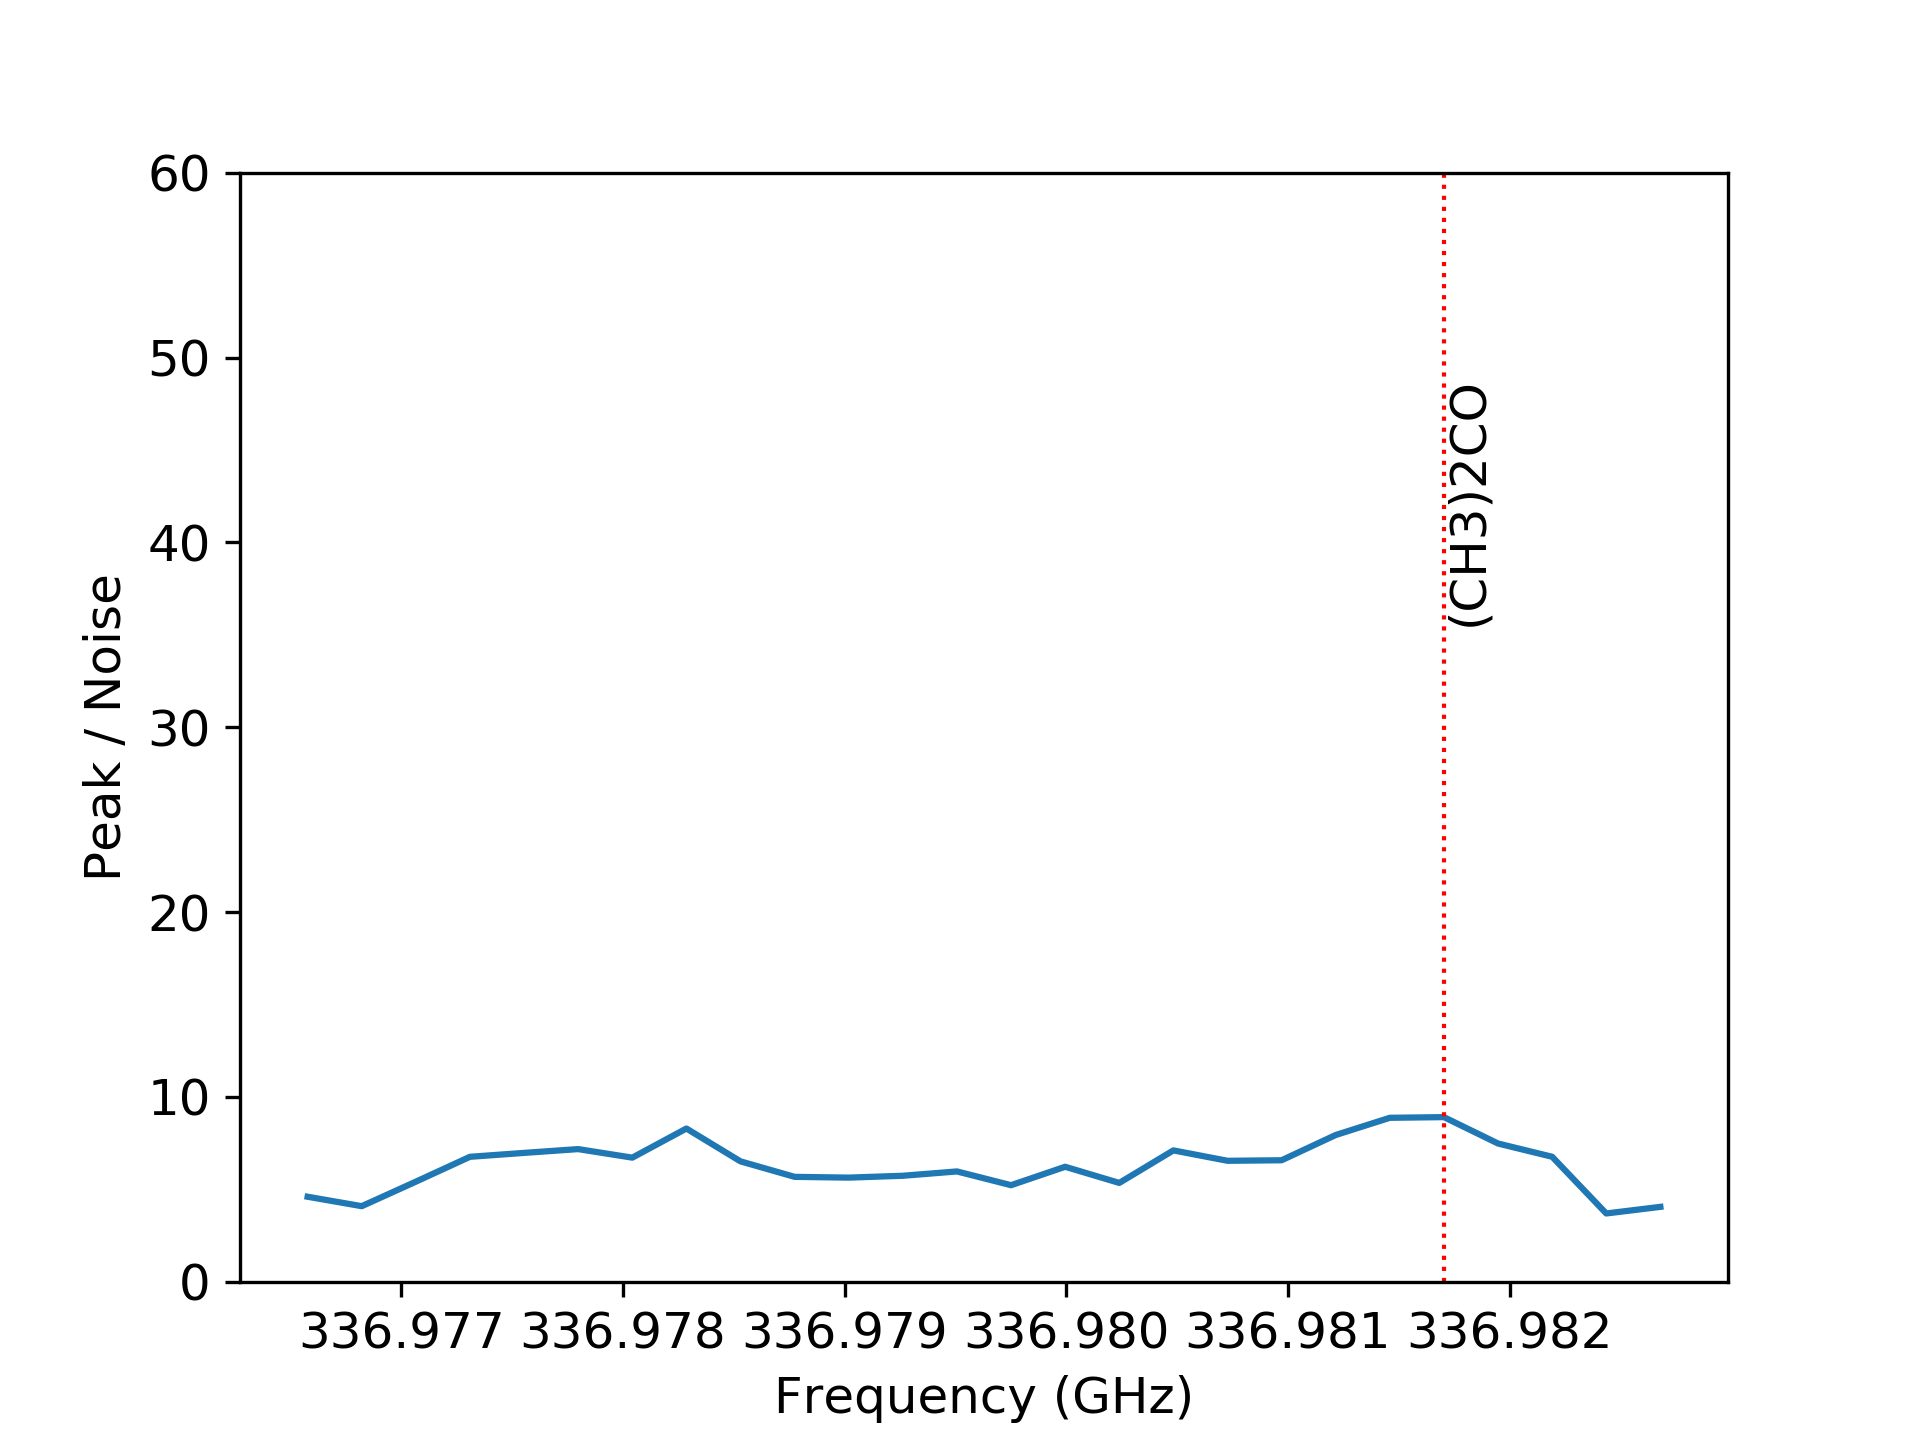
\includegraphics[width=0.33\textwidth]{spw0_(CH3)2CO}
    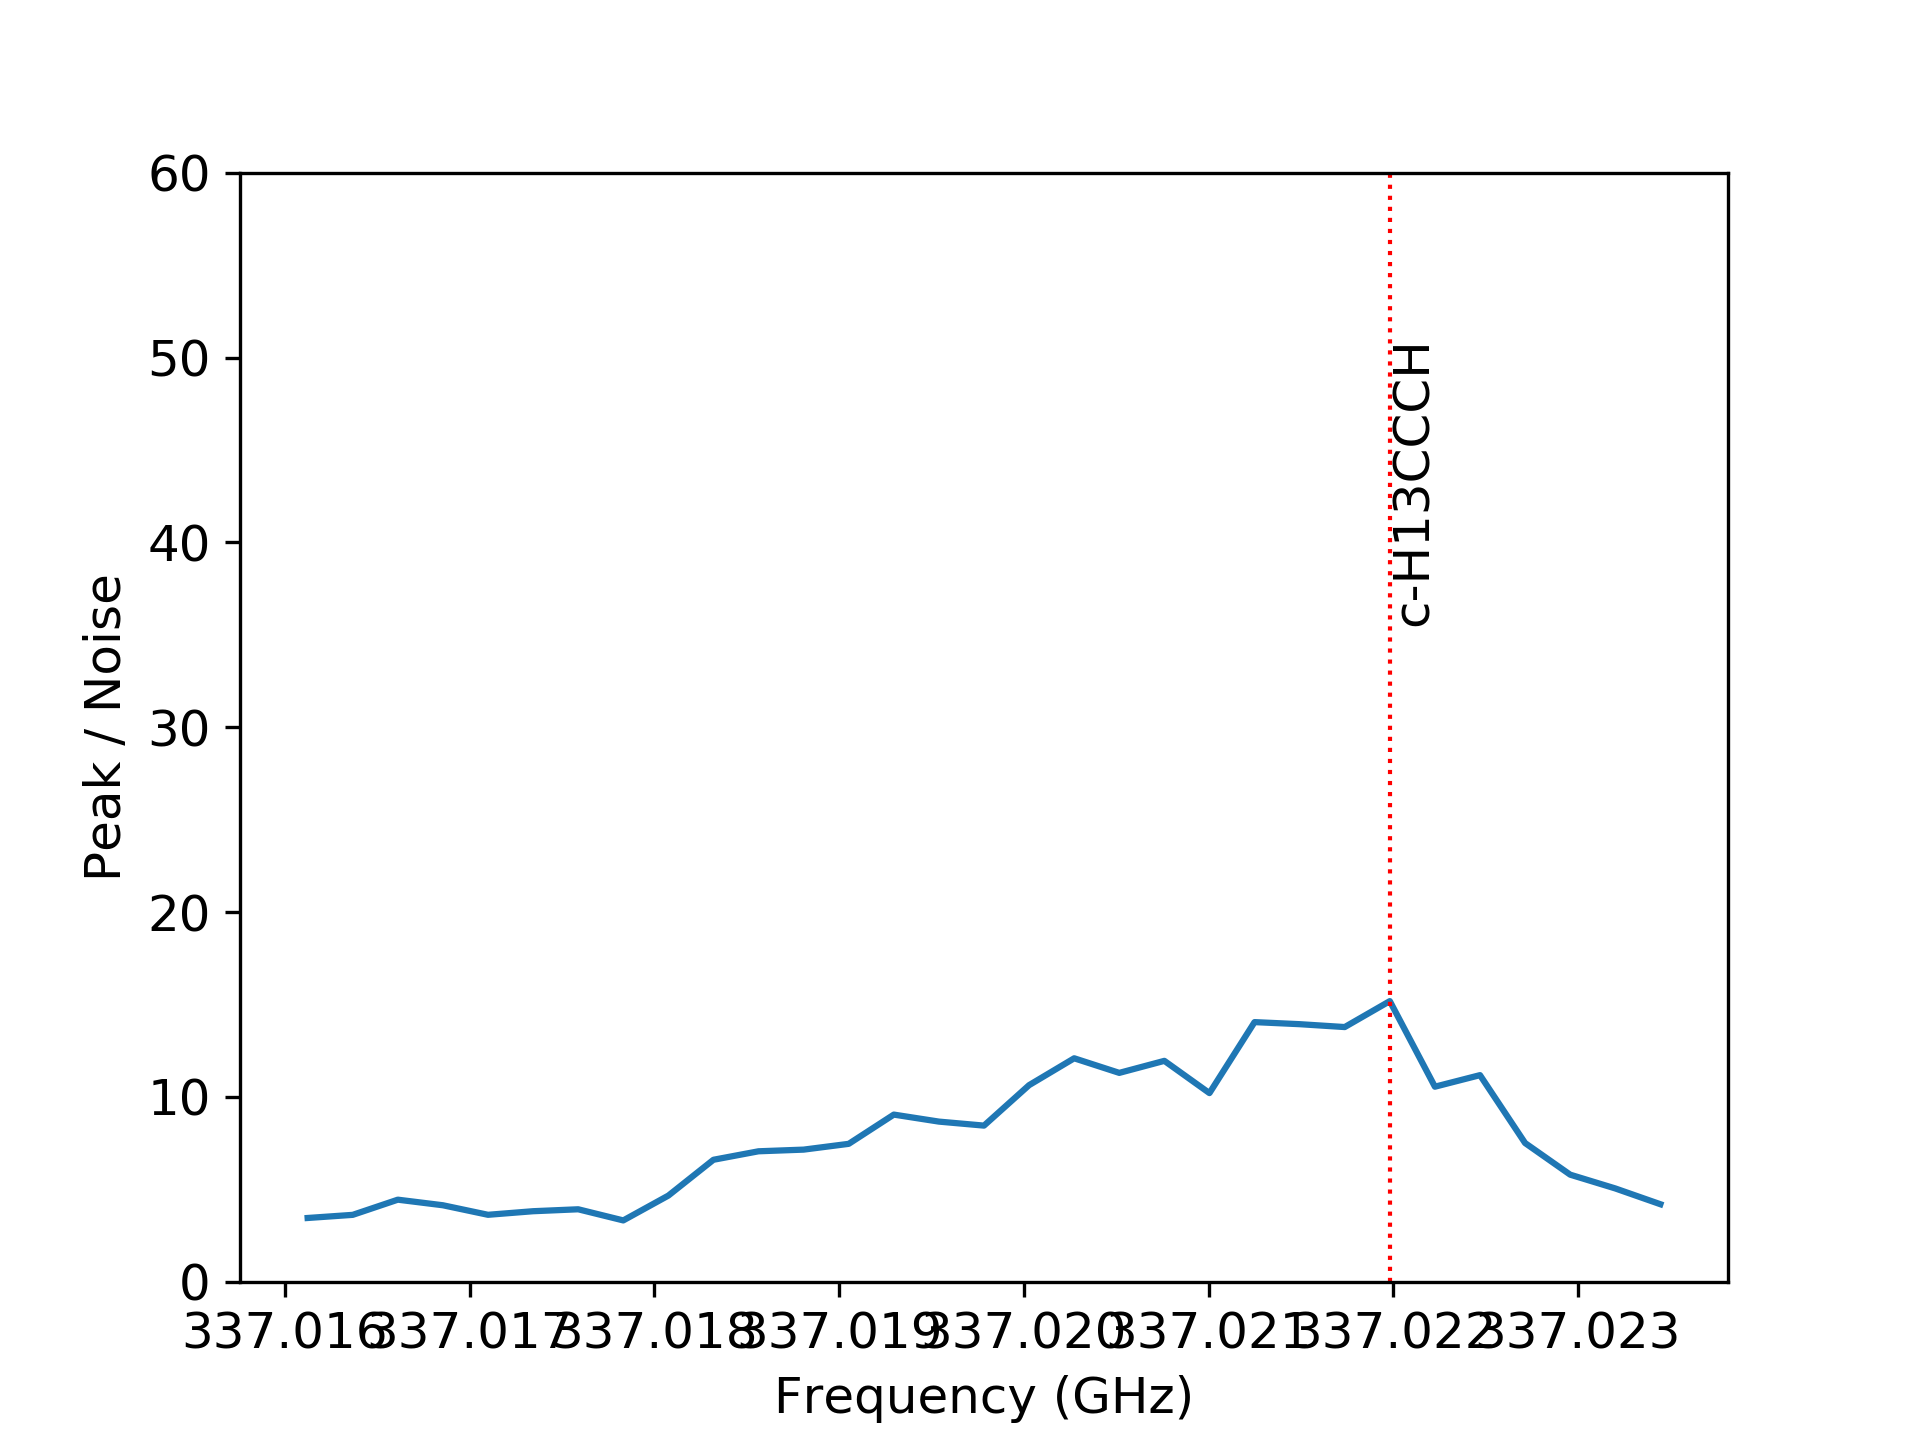
\includegraphics[width=0.33\textwidth]{spw0_c-H13CCCH}
    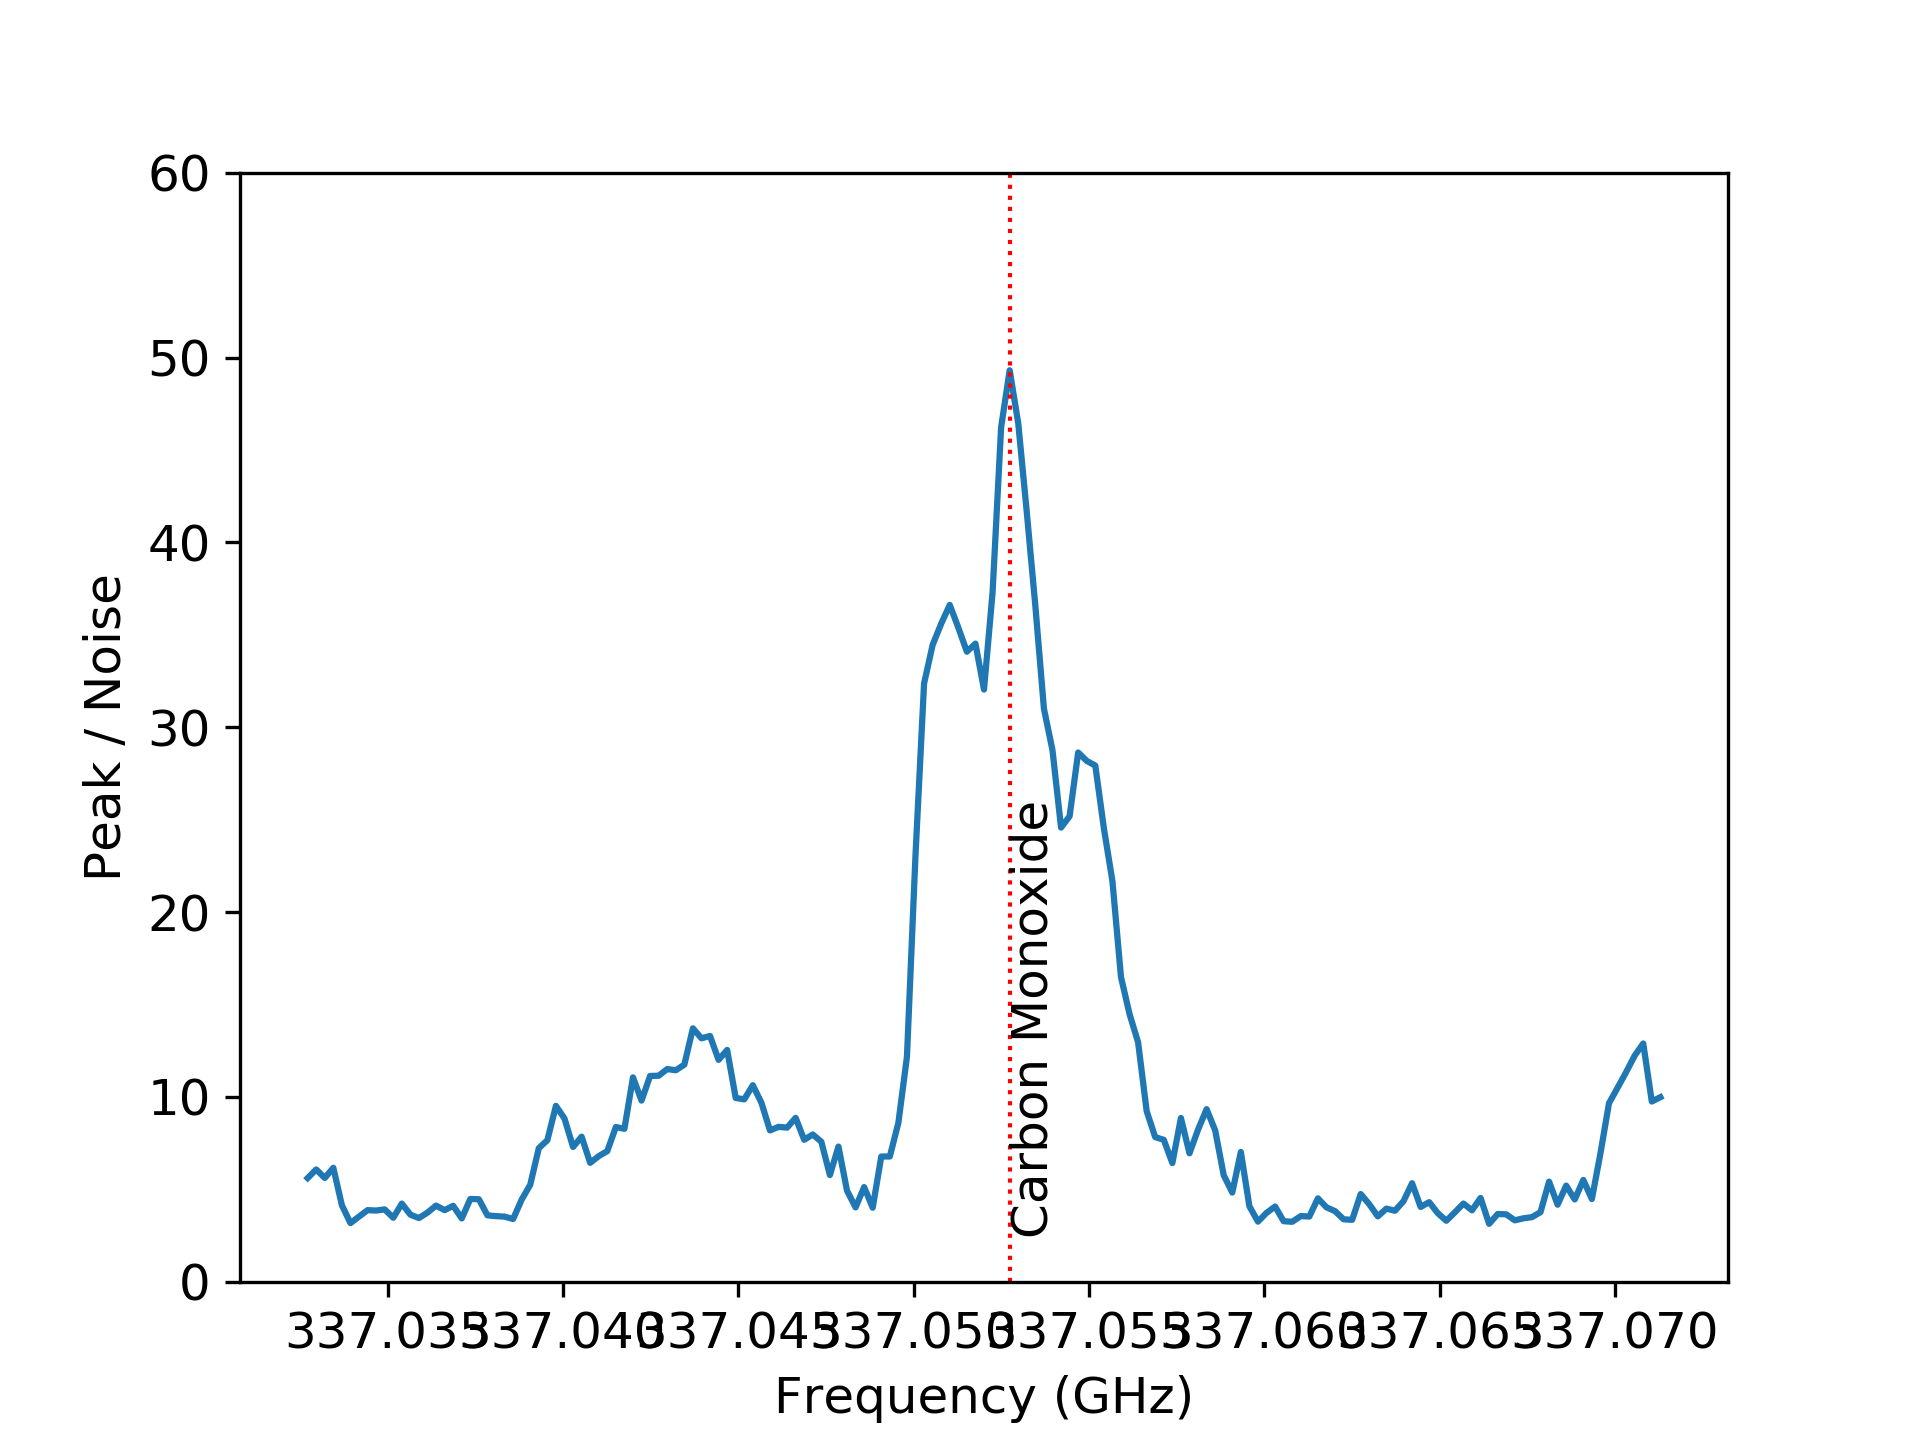
\includegraphics[width=0.33\textwidth]{spw0_C17O}
    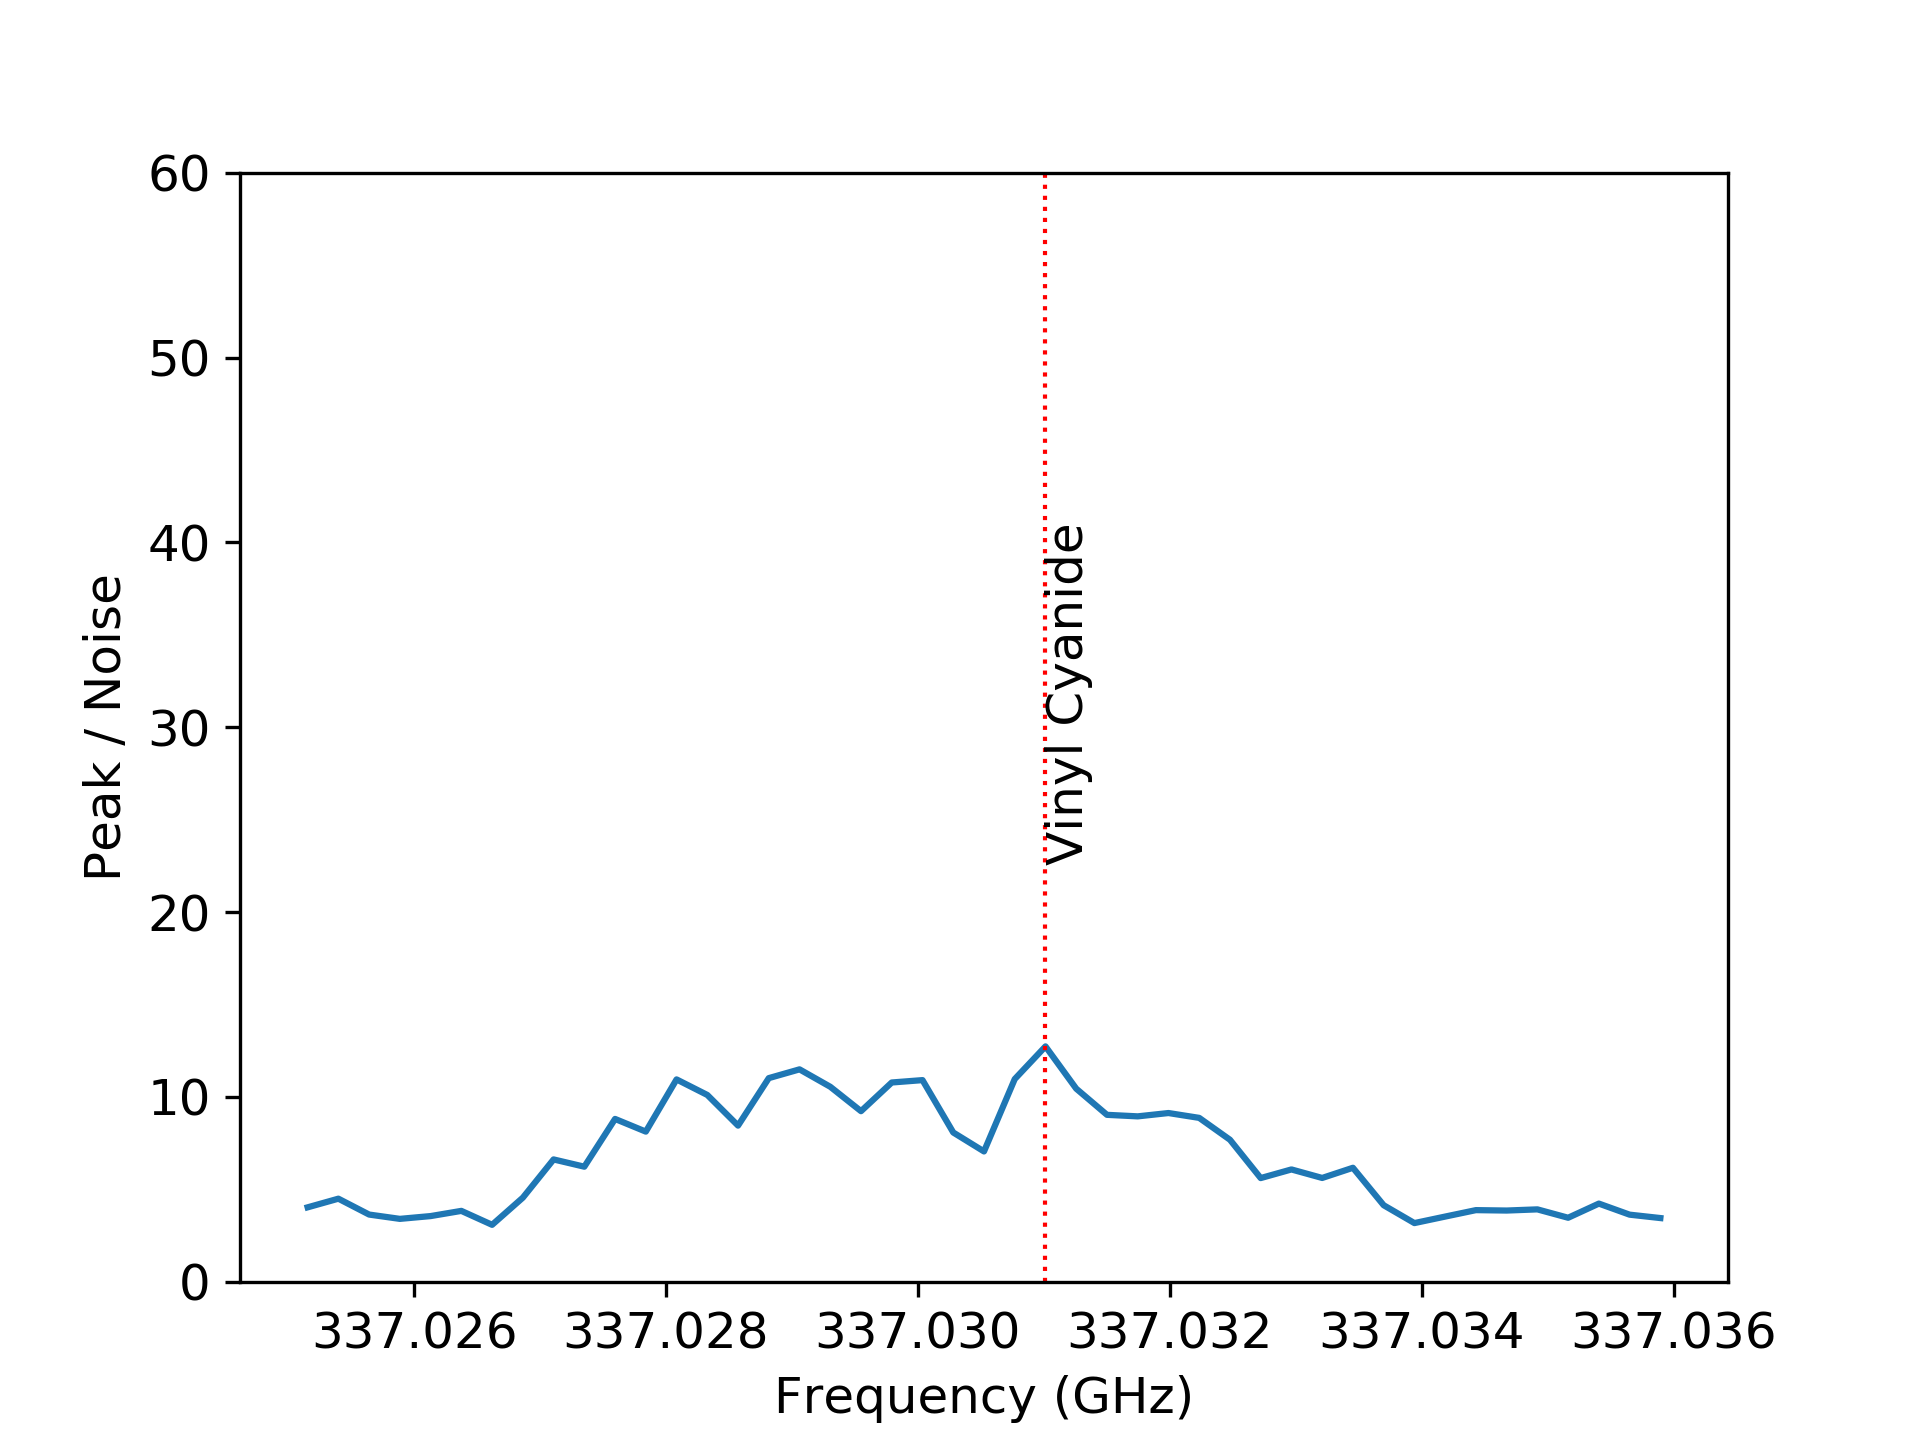
\includegraphics[width=0.33\textwidth]{spw0_CH2CHCN}
    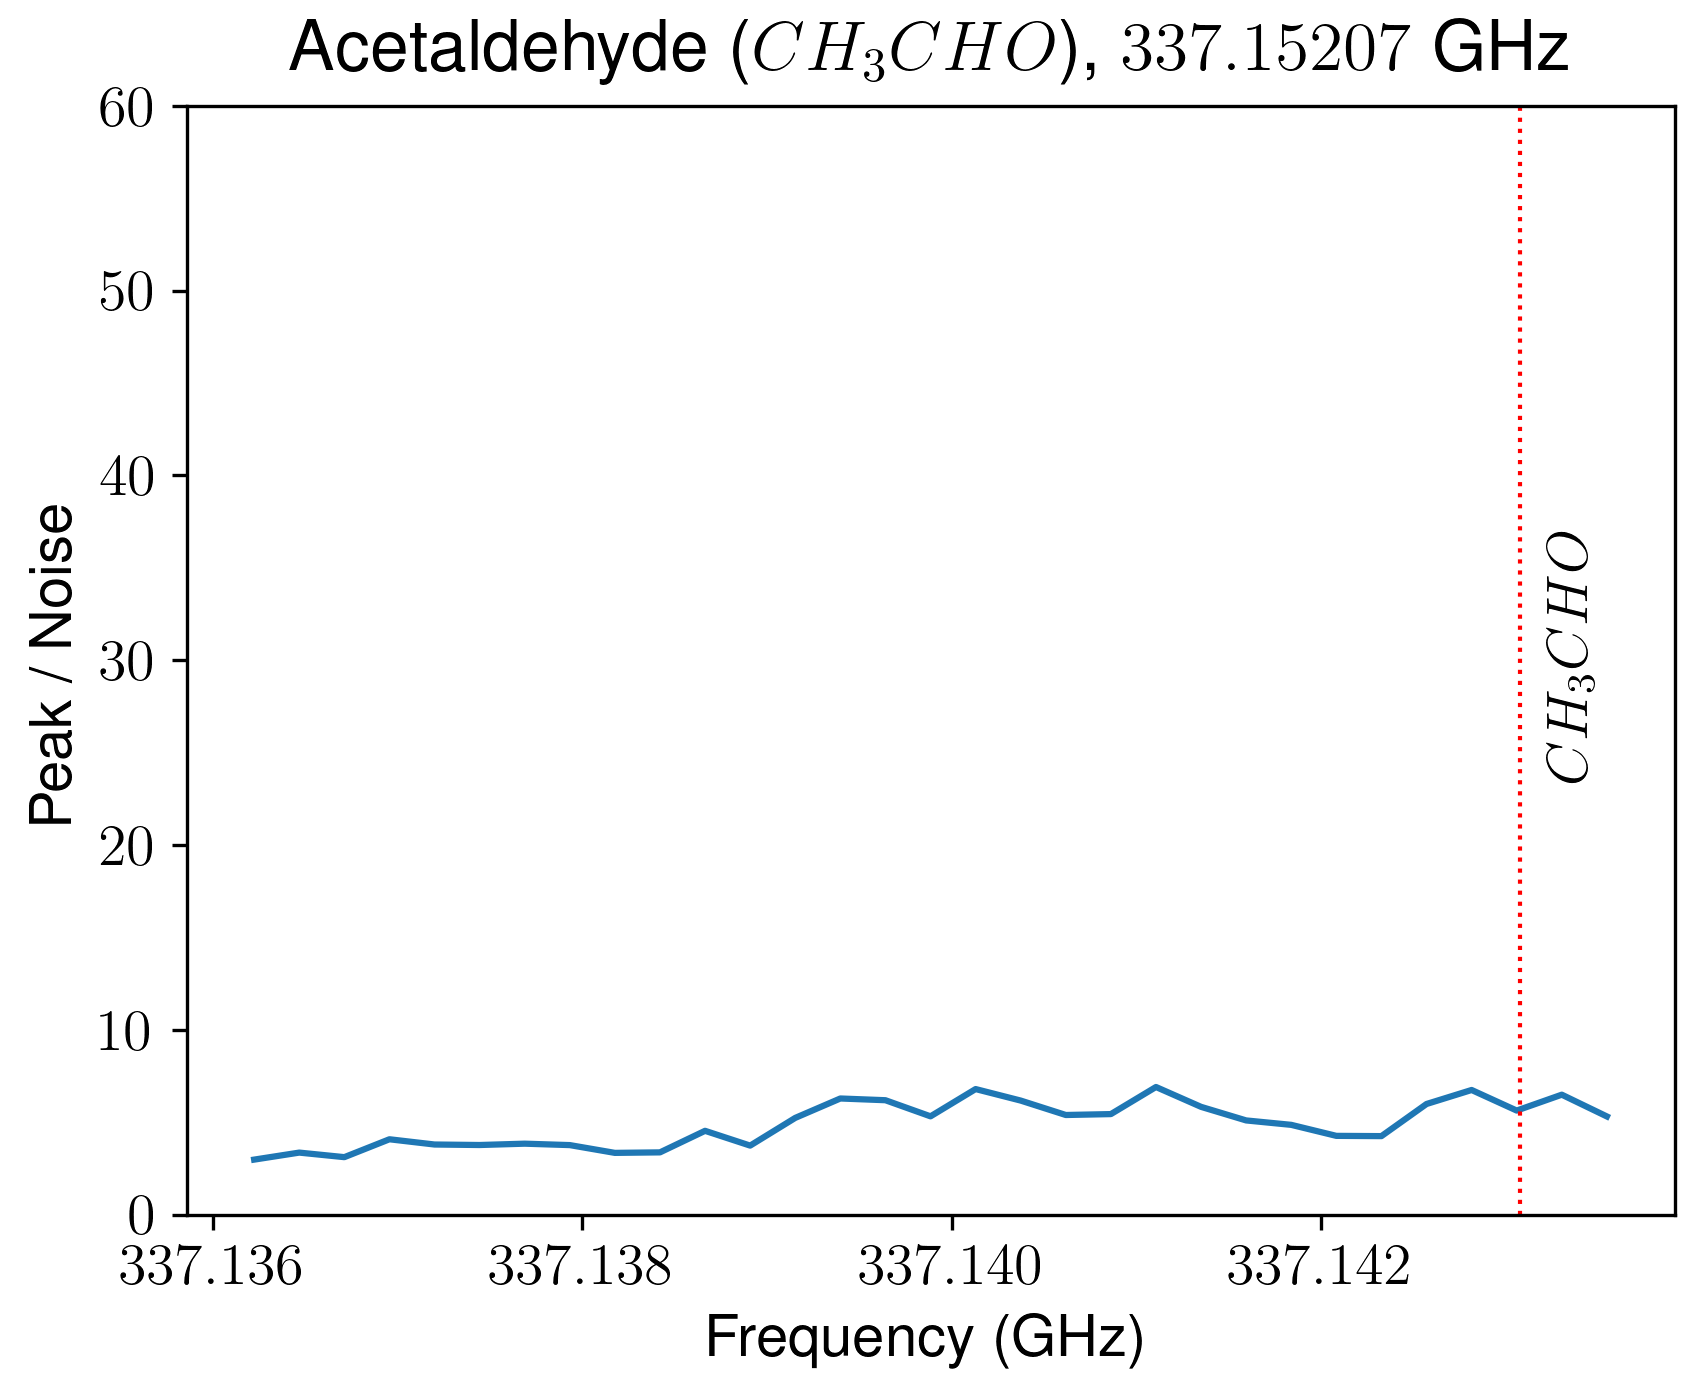
\includegraphics[width=0.33\textwidth]{spw0_CH3CHO}
    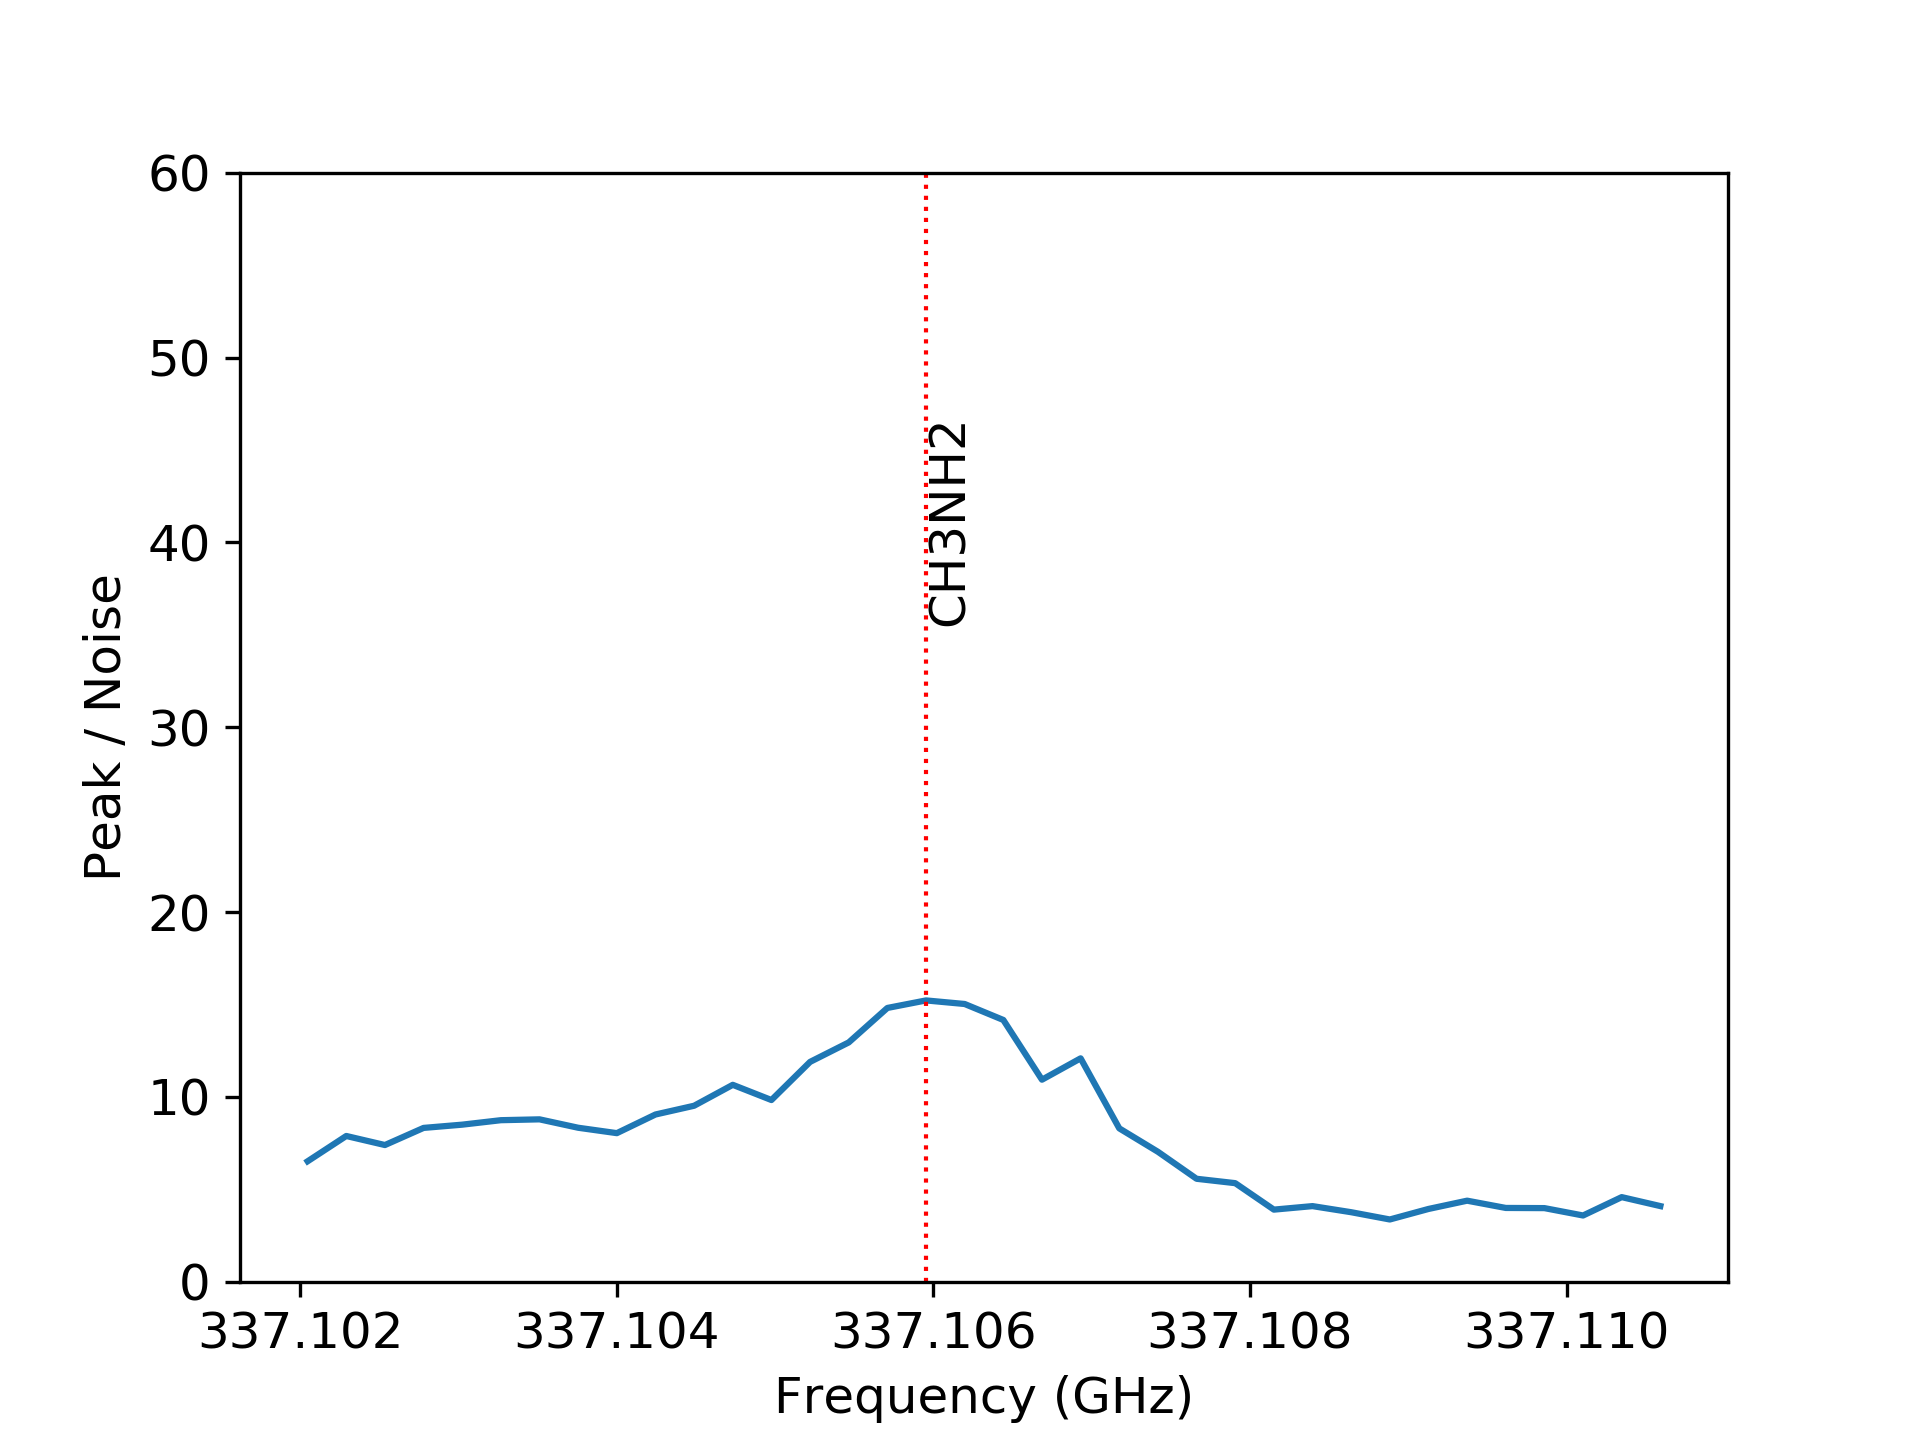
\includegraphics[width=0.33\textwidth]{spw0_CH3NH2}
    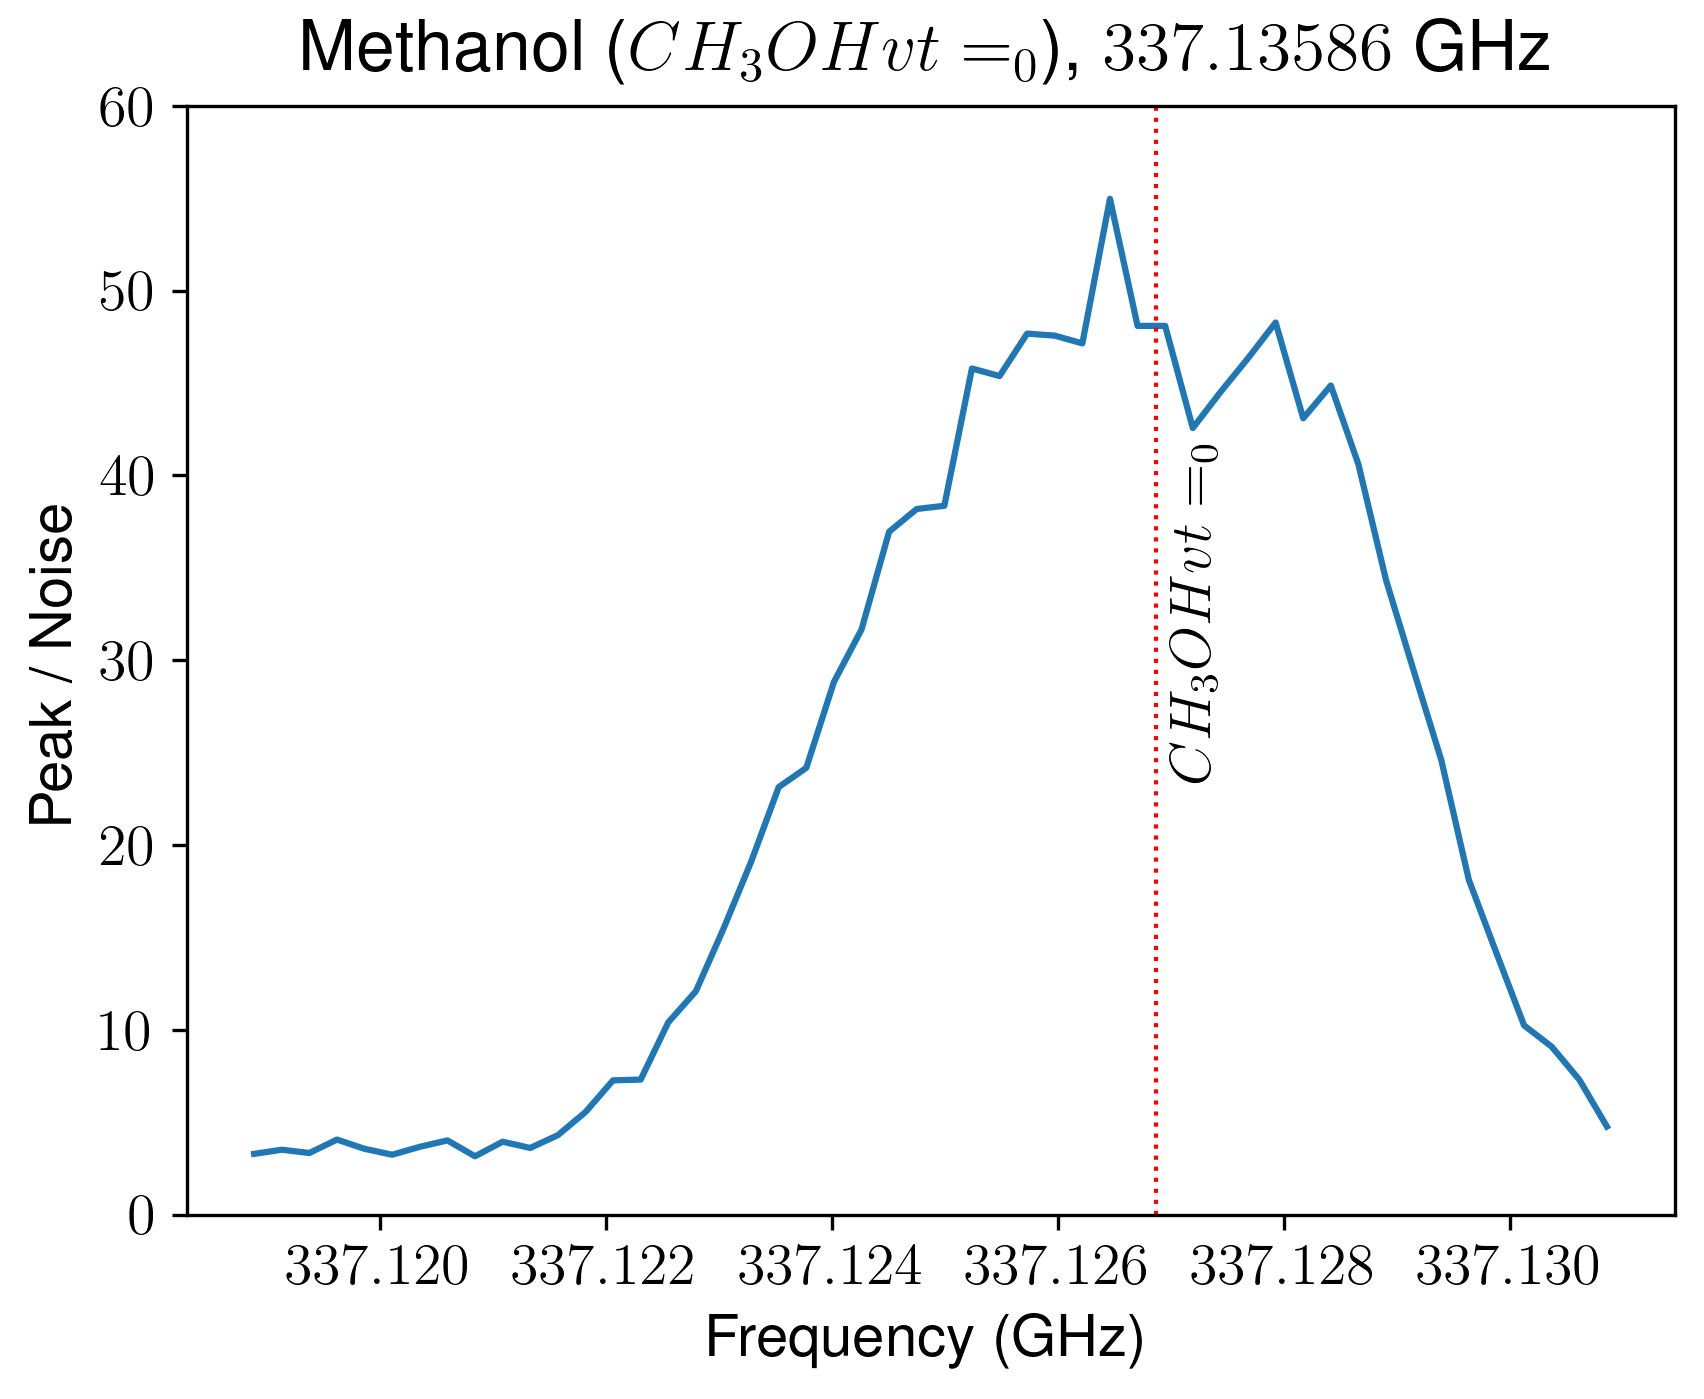
\includegraphics[width=0.33\textwidth]{spw0_CH3OHvt=0}
    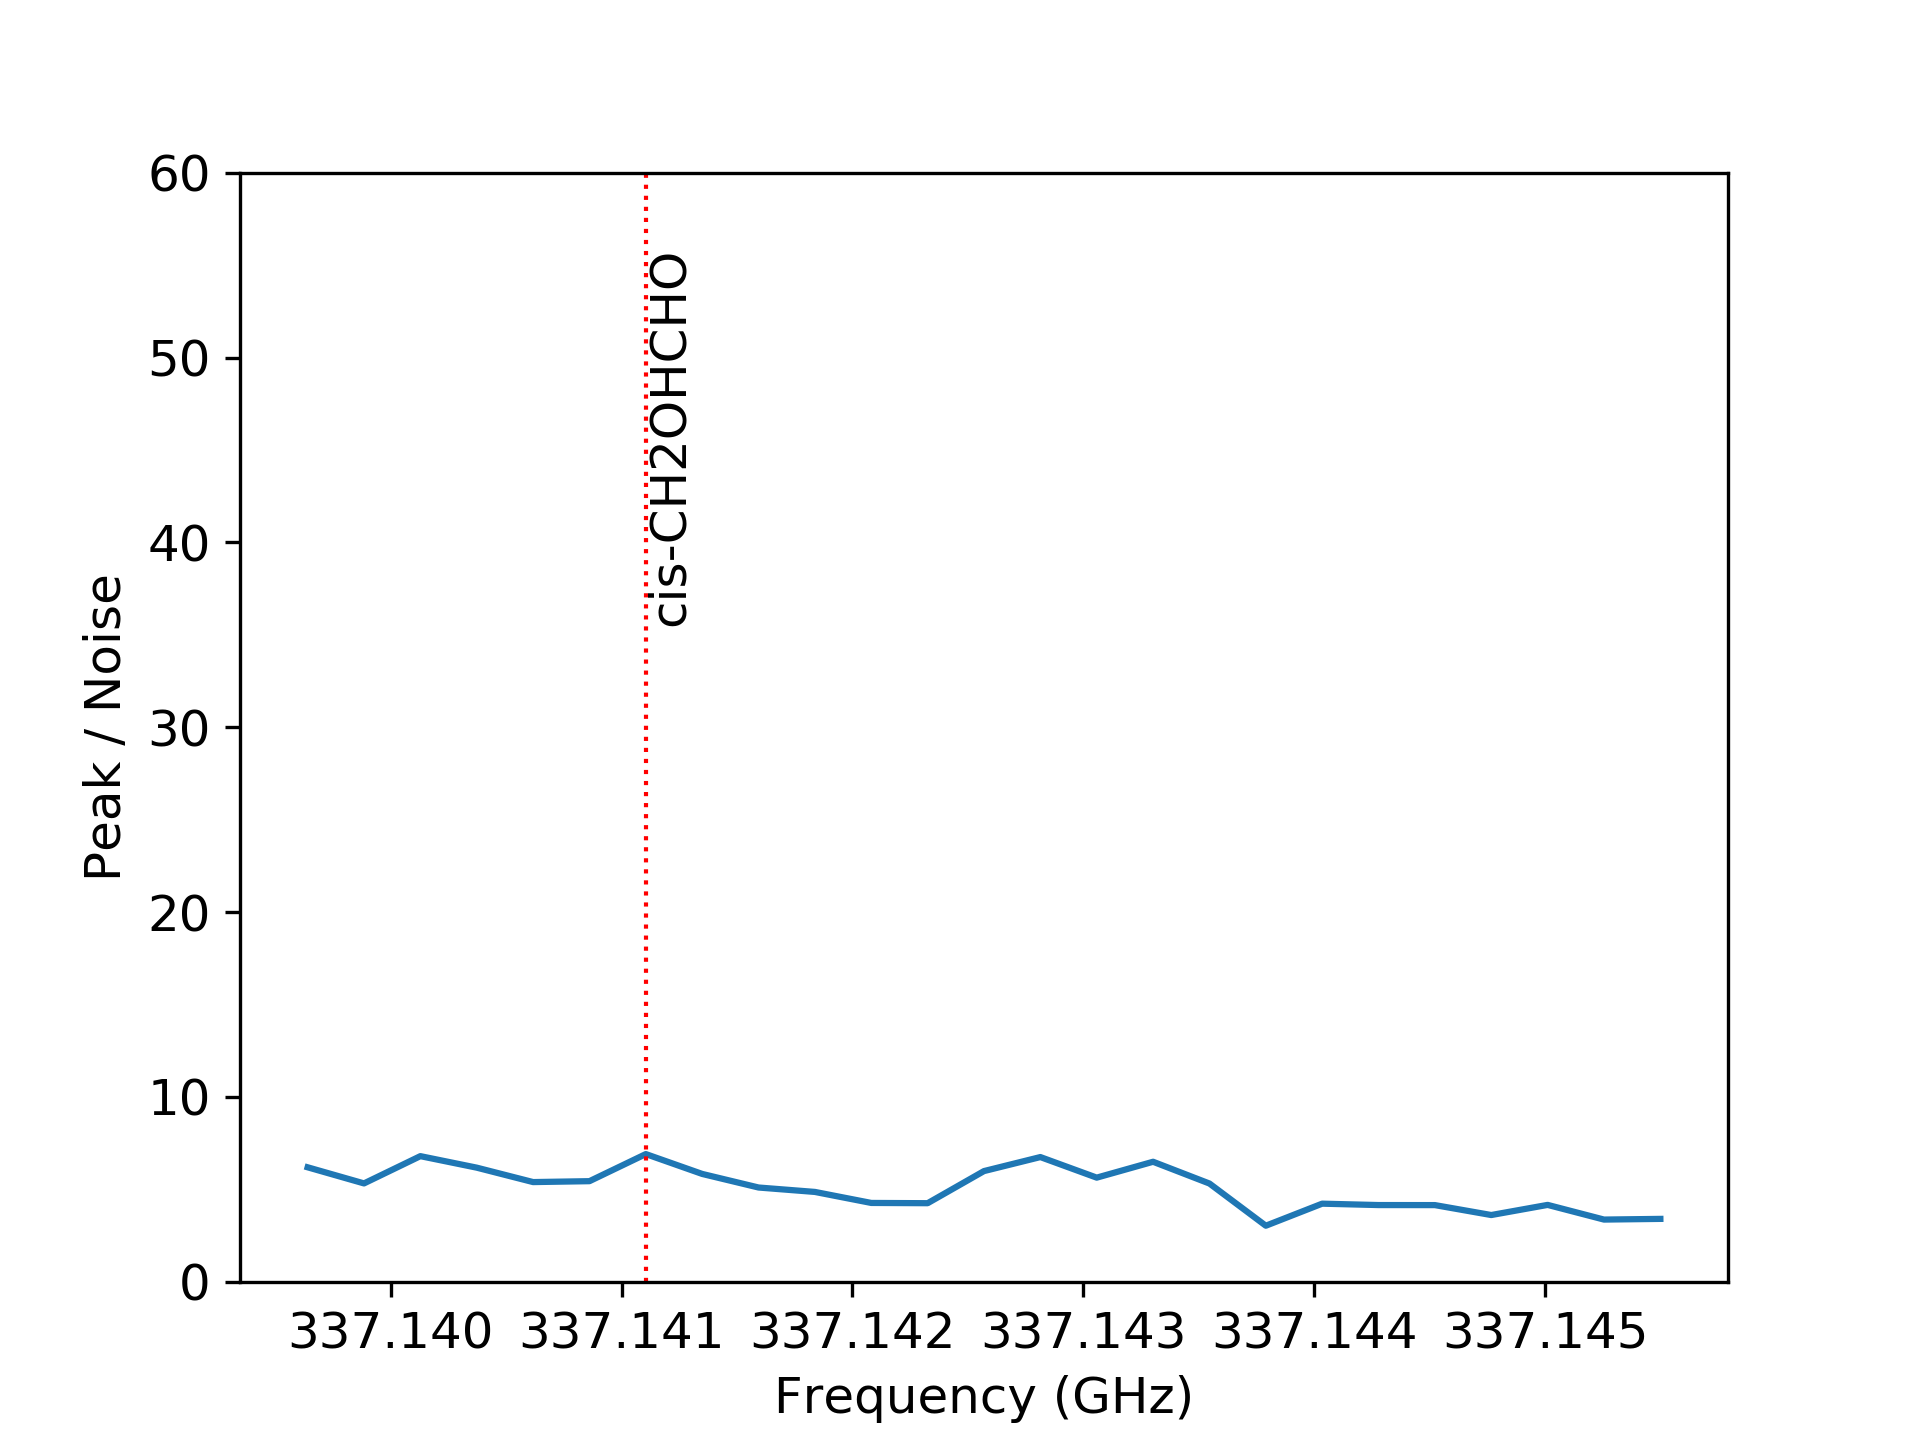
\includegraphics[width=0.33\textwidth]{spw0_cis-CH2OHCHO}
    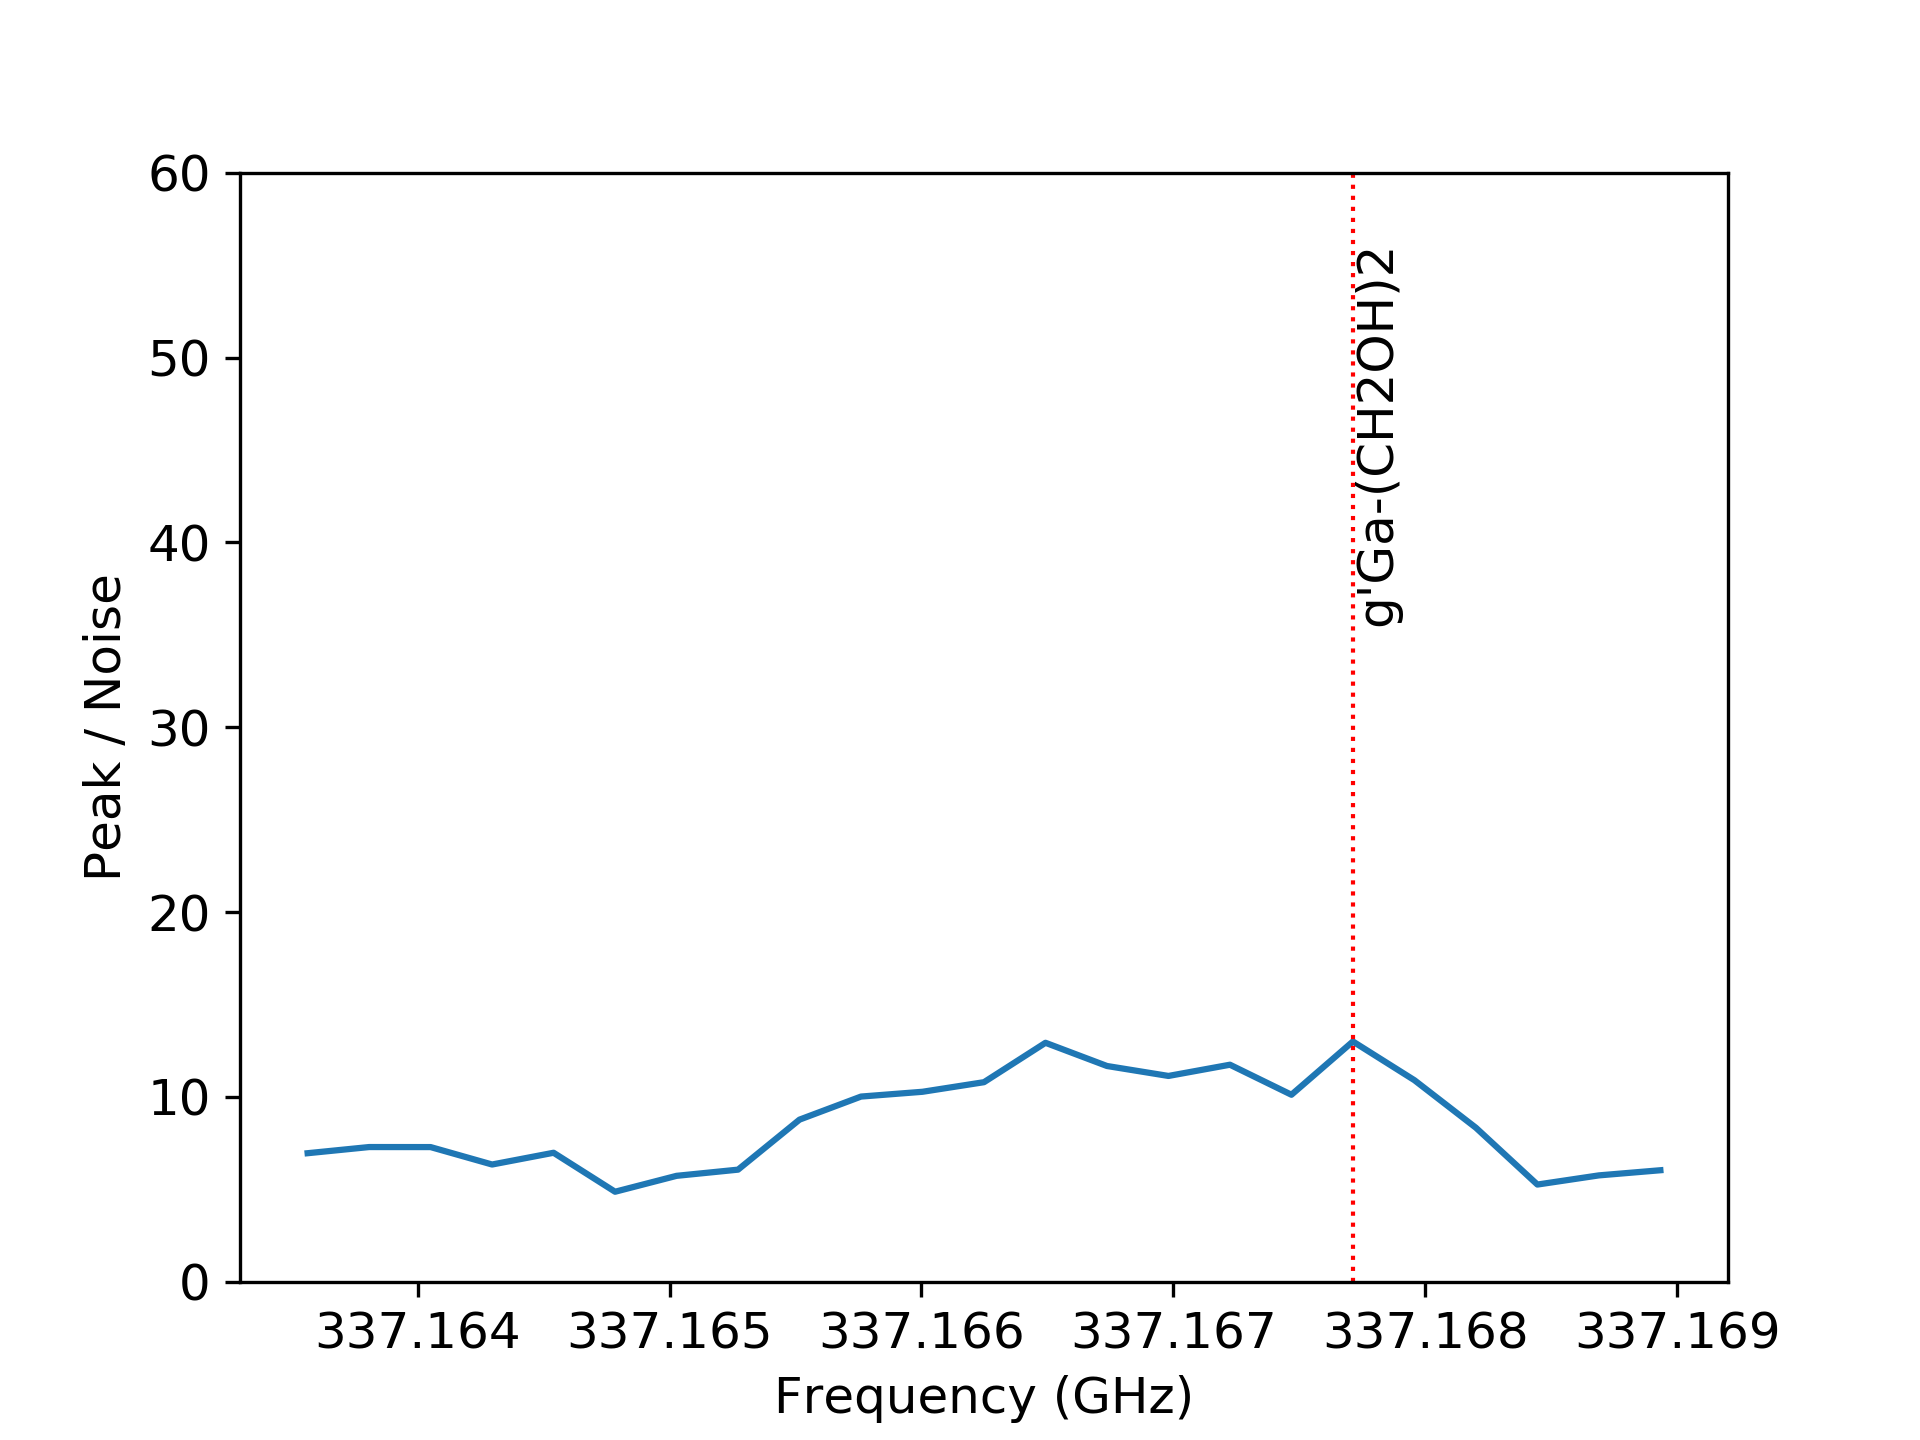
\includegraphics[width=0.33\textwidth]{spw0_g'Ga-(CH2OH)2}
    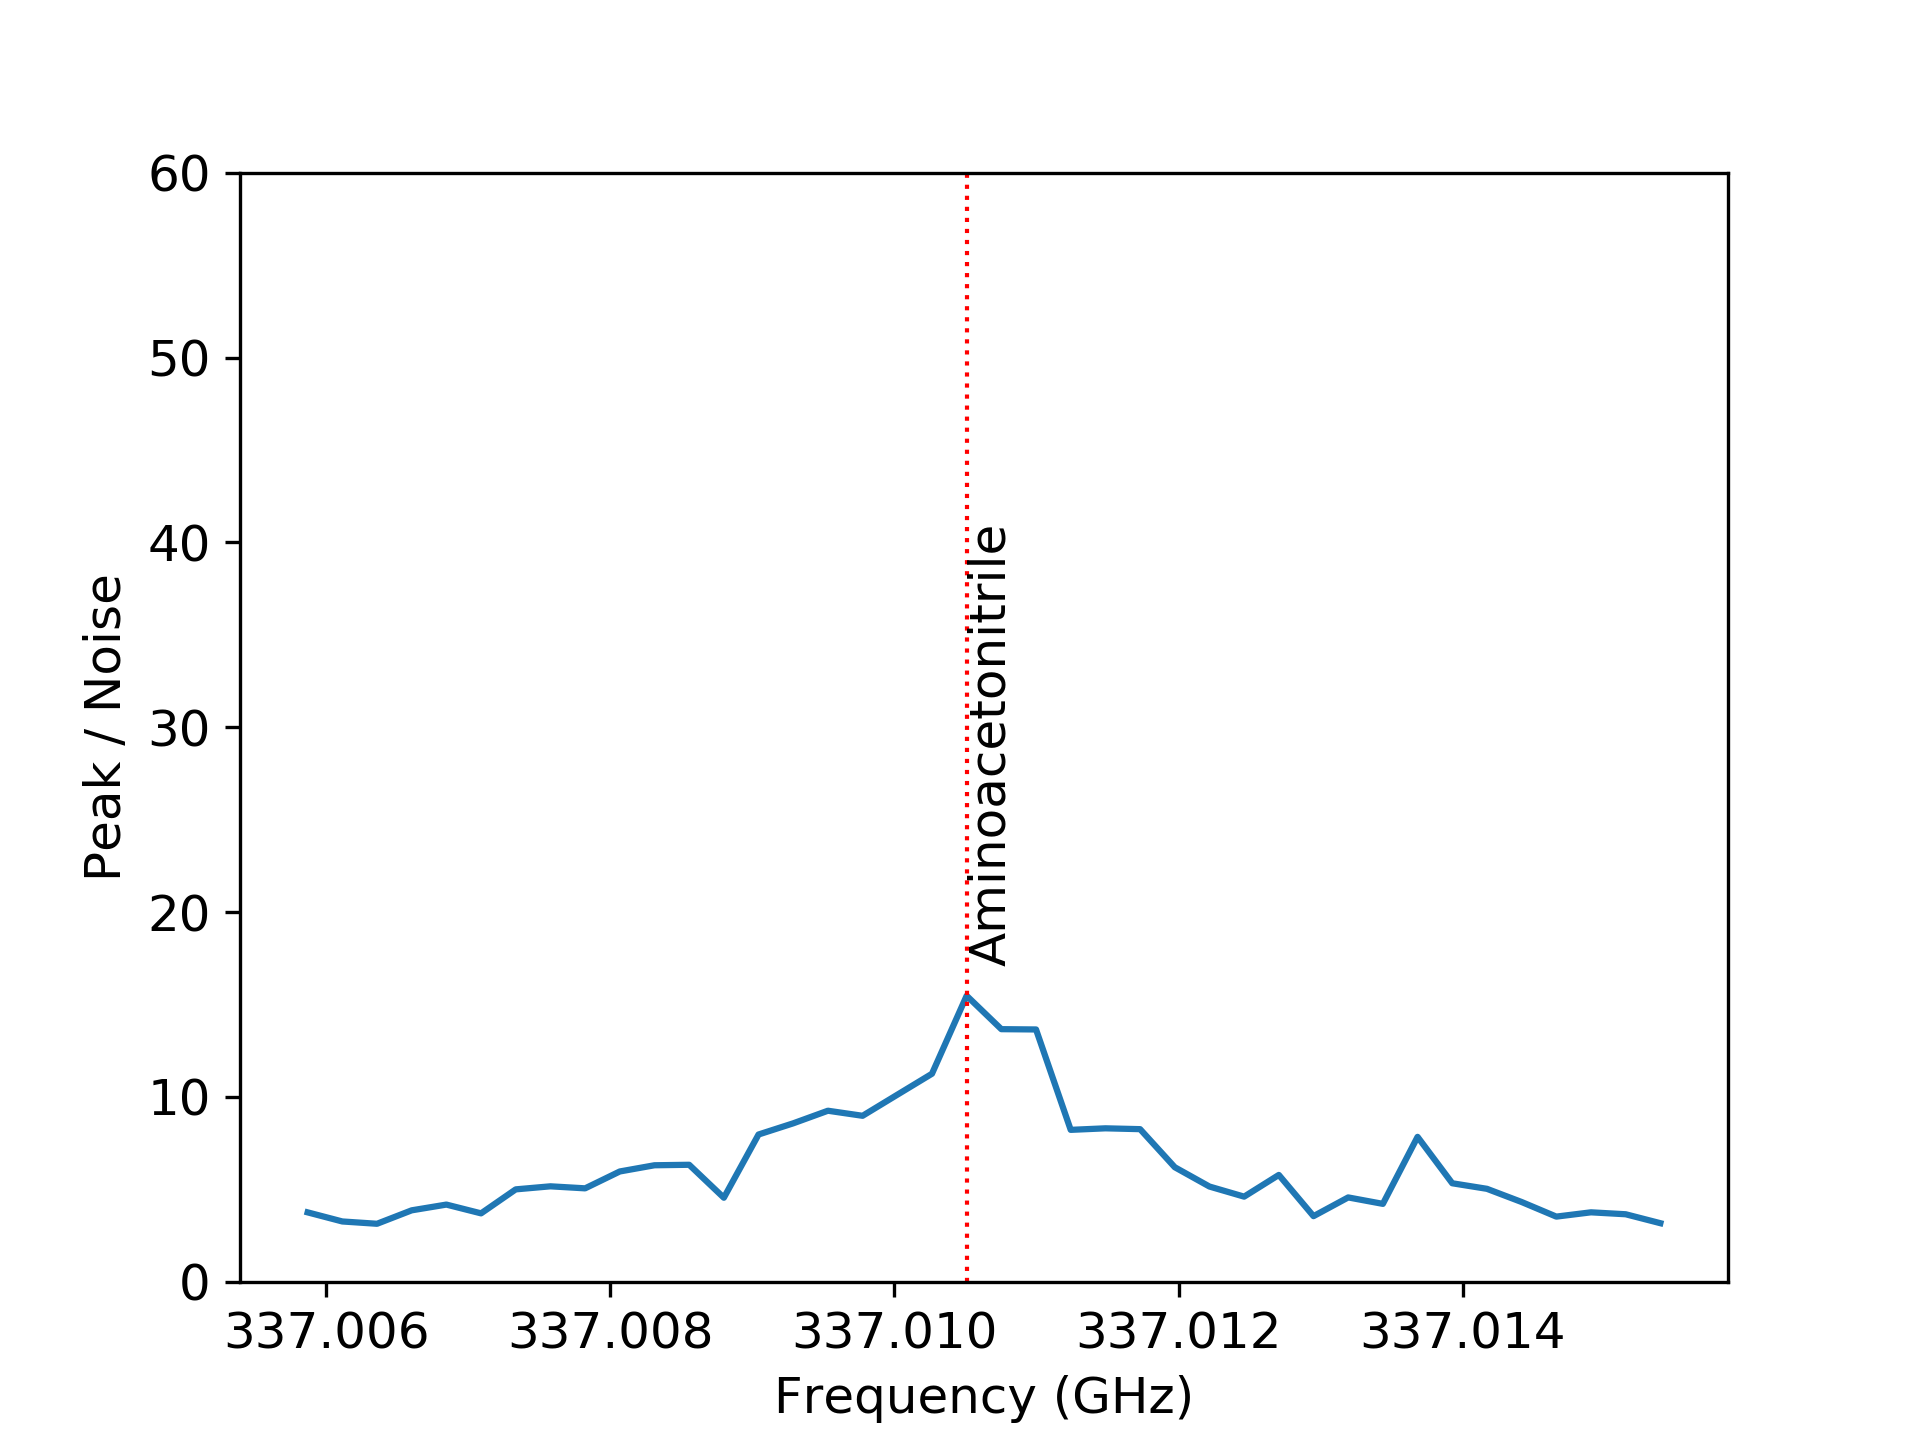
\includegraphics[width=0.33\textwidth]{spw0_H2NCH2CN}
    \caption{Promising molecular lines identified in spectral window 0}
   \end{figure*}
   
   \newpage
   \begin{table}[htb]  
    \caption{\textbf{Line identification results for spectral window 1}}
    \small
    \centering    
    \begin{tabular}{l l l l l l l l l} 
\hline
Molecule & Name & Transition & Frequency & $E_{{u}}$ & Intensity & Velocity & $V_{{lsr}}$ & peak / rms \\
\hline
$(CH_{3})_{2}COv=_{0}$ & Acetone & $33_{2,32}-32_{2,31}AE$ & $336.94769$ & $284.9779$ & $5.8645$ & $6.7346$ & $8.0$ & $8.2528$\\
$c-HCCCHv=_{0}$ & Cyclopropenylidene & $4_{4,1}-3_{1,2}$ & $336.94859$ & $32.2203$ & $7.7754$ & $8.5402$ & $8.0$ & $10.942$\\
$g'Ga-(CH_{2}OH)_{2}$ & Ethylene Glycol & $29_{17,12}v=0-29_{16,13}v=0$ & $336.95735$ & $355.5986$ & $22.9795$ & $7.6964$ & $8.0$ & $32.3382$\\
$(CH_{3})_{2}COv=_{0}$ & Acetone & $33_{1,32}-32_{2,31}EE$ & $336.96839$ & $284.9042$ & $8.6102$ & $8.9506$ & $8.0$ & $12.1167$\\
$(CH_{3})_{2}COv=_{0}$ & Acetone & $24_{12,13}-23_{11,12}EE$ & $336.97681$ & $230.3935$ & $2.1859$ & $6.0204$ & $8.0$ & $3.0761$\\
$(CH_{3})_{2}COv=_{0}$ & Acetone & $33_{1,32}-32_{2,31}AA$ & $336.98907$ & $284.8304$ & $3.5648$ & $9.0125$ & $8.0$ & $5.0166$\\
$H_{2}NCH_{2}CN$ & Aminoacetonitrile & $37_{5,33}-36_{5,32}$ & $337.01833$ & $337.6508$ & $8.1389$ & $8.8251$ & $8.0$ & $11.4536$\\
$g-CH_{3}CH_{2}OH$ & gauche-Ethanol & $36_{5,32}-35_{6,29},vt=0-0$ & $337.02461$ & $643.1397$ & $8.0259$ & $13.0103$ & $8.0$ & $11.2946$\\
$c-H_{13}CCCH$ & Cyclopropenylidene & $21_{11,10}-21_{11,11}$ & $337.02915$ & $649.5308$ & $0.0$ & $0.0$ & $8.0$ & $0.0$\\
$CH_{2}CHCNv=_{0}$ & Vinyl Cyanide & $36_{2,35}-35_{2,34}$ & $337.03974$ & $309.7482$ & $6.3892$ & $7.3691$ & $8.0$ & $8.9912$\\
$C_{17}O$ & Carbon Monoxide & $J=3-2$ & $337.0611$ & $32.3538$ & $32.425$ & $0.5295$ & $8.0$ & $45.6304$\\
$g'Ga-(CH_{2}OH)_{2}$ & Ethylene Glycol & $33_{8,25}v=0-32_{8,24}v=1$ & $337.08211$ & $309.0677$ & $6.6297$ & $5.9492$ & $8.0$ & $9.3296$\\
$cis-CH_{2}OHCHOv=_{0}$ & Glycolaldehyde & $29_{13,17}-28_{13,16}$ & $337.09926$ & $344.463$ & $20.9463$ & $7.5278$ & $8.0$ & $29.4769$\\
$cis-CH_{2}OHCHOv=_{0}$ & Glycolaldehyde & $29_{13,16}-28_{13,15}$ & $337.09927$ & $344.463$ & $0.0$ & $0.0$ & $8.0$ & $0.0$\\
$g'Ga-(CH_{2}OH)_{2}$ & Ethylene Glycol & $69_{18,52}v=1-69_{17,53}v=1$ & $337.10336$ & $1346.196$ & $-0.0118$ & $8.1634$ & $8.0$ & $-2.8258$\\
$CH_{3}NH_{2}$ & Methylamine & $2_{2}E2-1-1_{1}E2-1,F=2-2$ & $337.11864$ & $22.2636$ & $0.0$ & $0.0$ & $8.0$ & $0.0$\\
$CH_{3}NH_{2}$ & Methylamine & $2_{2}E2-1-1_{1}E2-1,F=2-1$ & $337.11894$ & $22.2636$ & $8.052$ & $3.7404$ & $8.0$ & $11.3313$\\
$CH_{3}OHvt=_{0}$ & Methanol & $3_{3,0}-4_{2,2}$ & $337.13586$ & $61.6392$ & $36.2978$ & $7.6565$ & $8.0$ & $51.0804$\\
$cis-CH_{2}OHCHOv=_{0}$ & Glycolaldehyde & $15_{7,9}-14_{6,8}$ & $337.15086$ & $96.4924$ & $2.1438$ & $7.3493$ & $8.0$ & $3.0169$\\
$CH_{3}CHOv=_{0}$ & Acetaldehyde & $13_{1,12}-12_{-1,12}E$ & $337.15207$ & $88.4514$ & $0.0247$ & $6.2404$ & $8.0$ & $5.9389$\\
$g'Ga-(CH_{2}OH)_{2}$ & Ethylene Glycol & $26_{17,9}v=1-26_{16,10}v=1$ & $337.16832$ & $314.6439$ & $0.0147$ & $7.4294$ & $8.0$ & $3.5352$\\
$g'Ga-(CH_{2}OH)_{2}$ & Ethylene Glycol & $24_{17,7}v=0-24_{16,8}v=0$ & $337.17585$ & $289.264$ & $0.0$ & $0.0$ & $8.0$ & $0.0$\\
\hline
                
    \end{tabular}
\end{table}

\newpage
   \begin{figure*}
    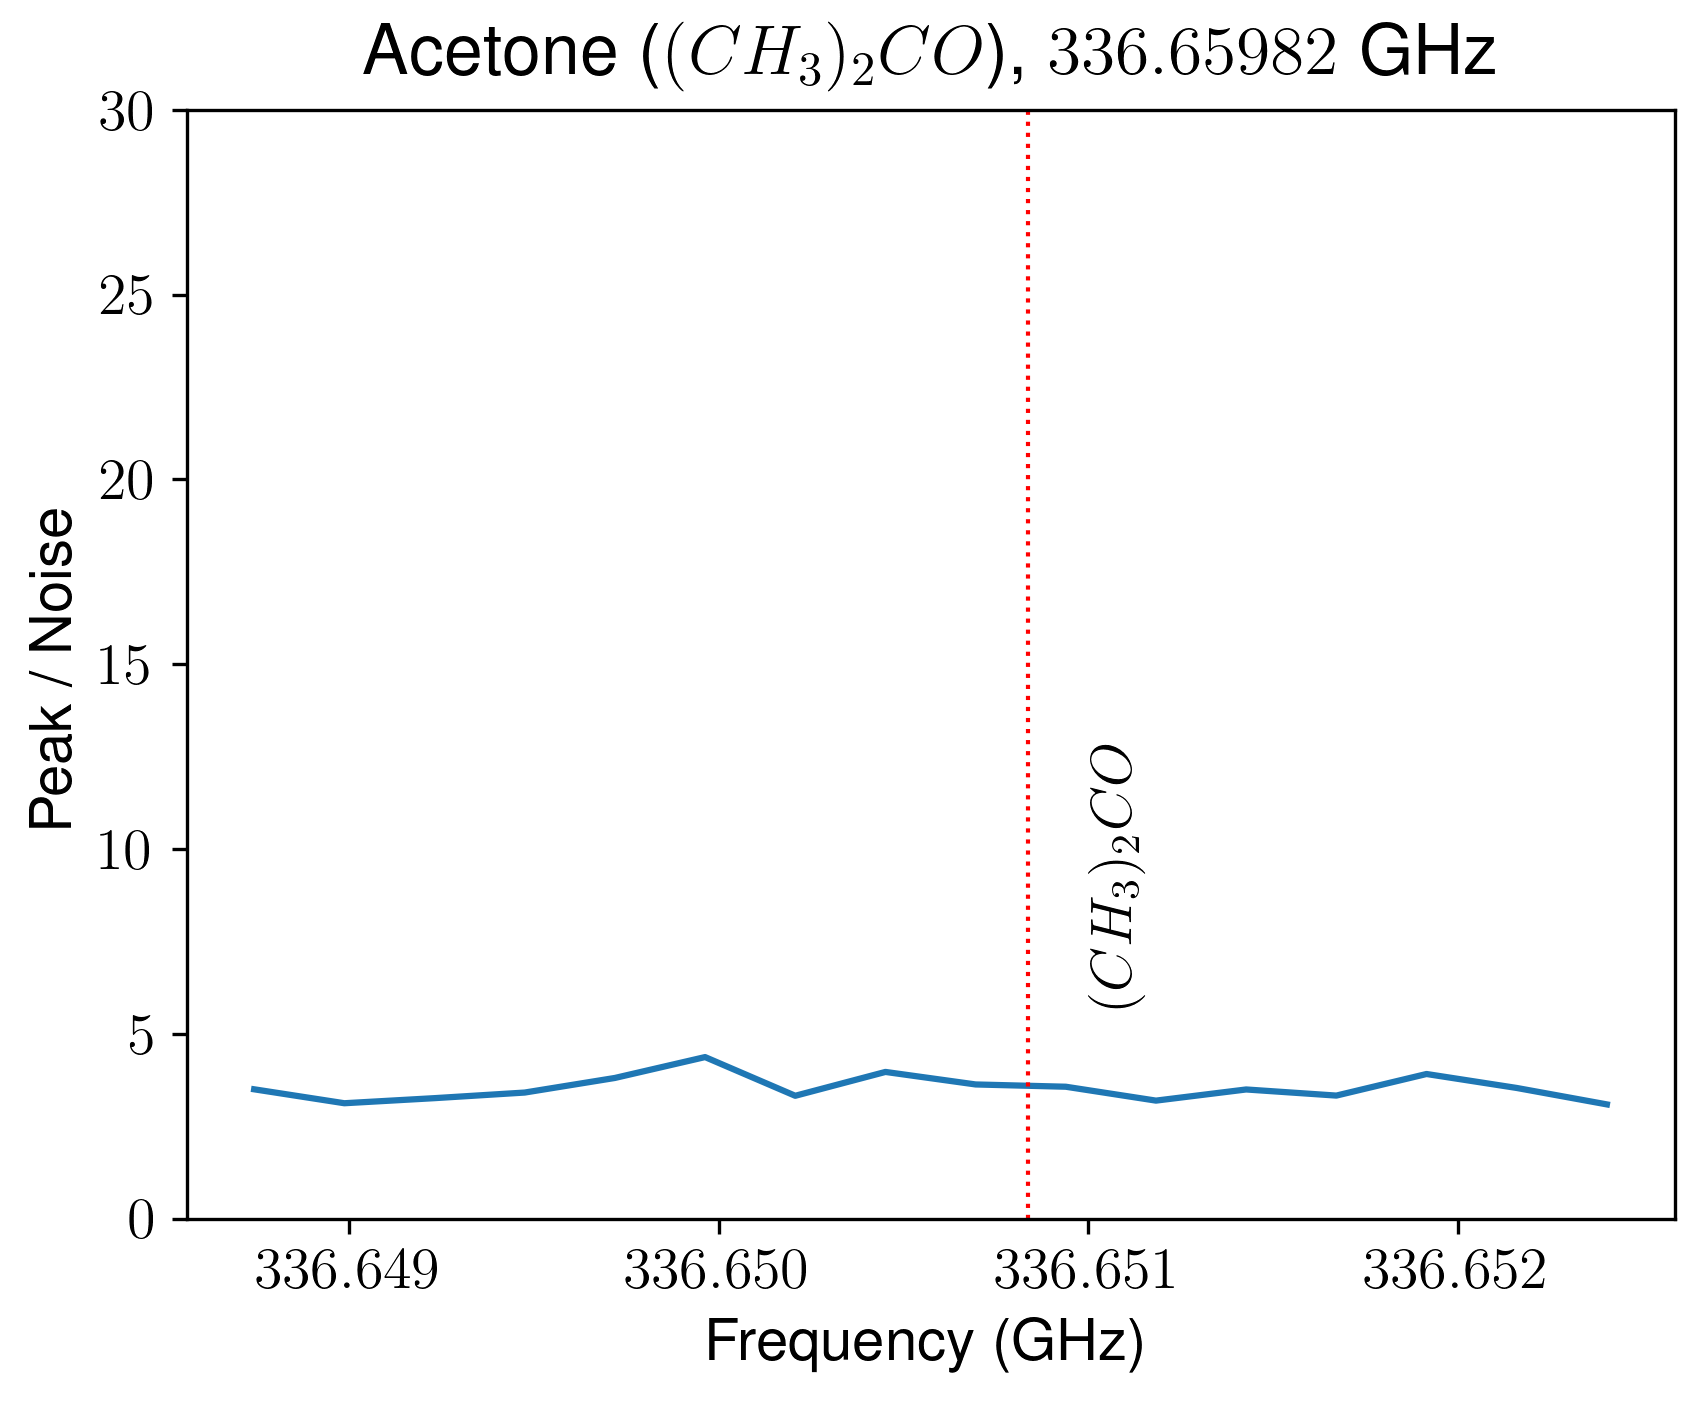
\includegraphics[width=0.33\textwidth]{spw1_(CH3)2CO}
    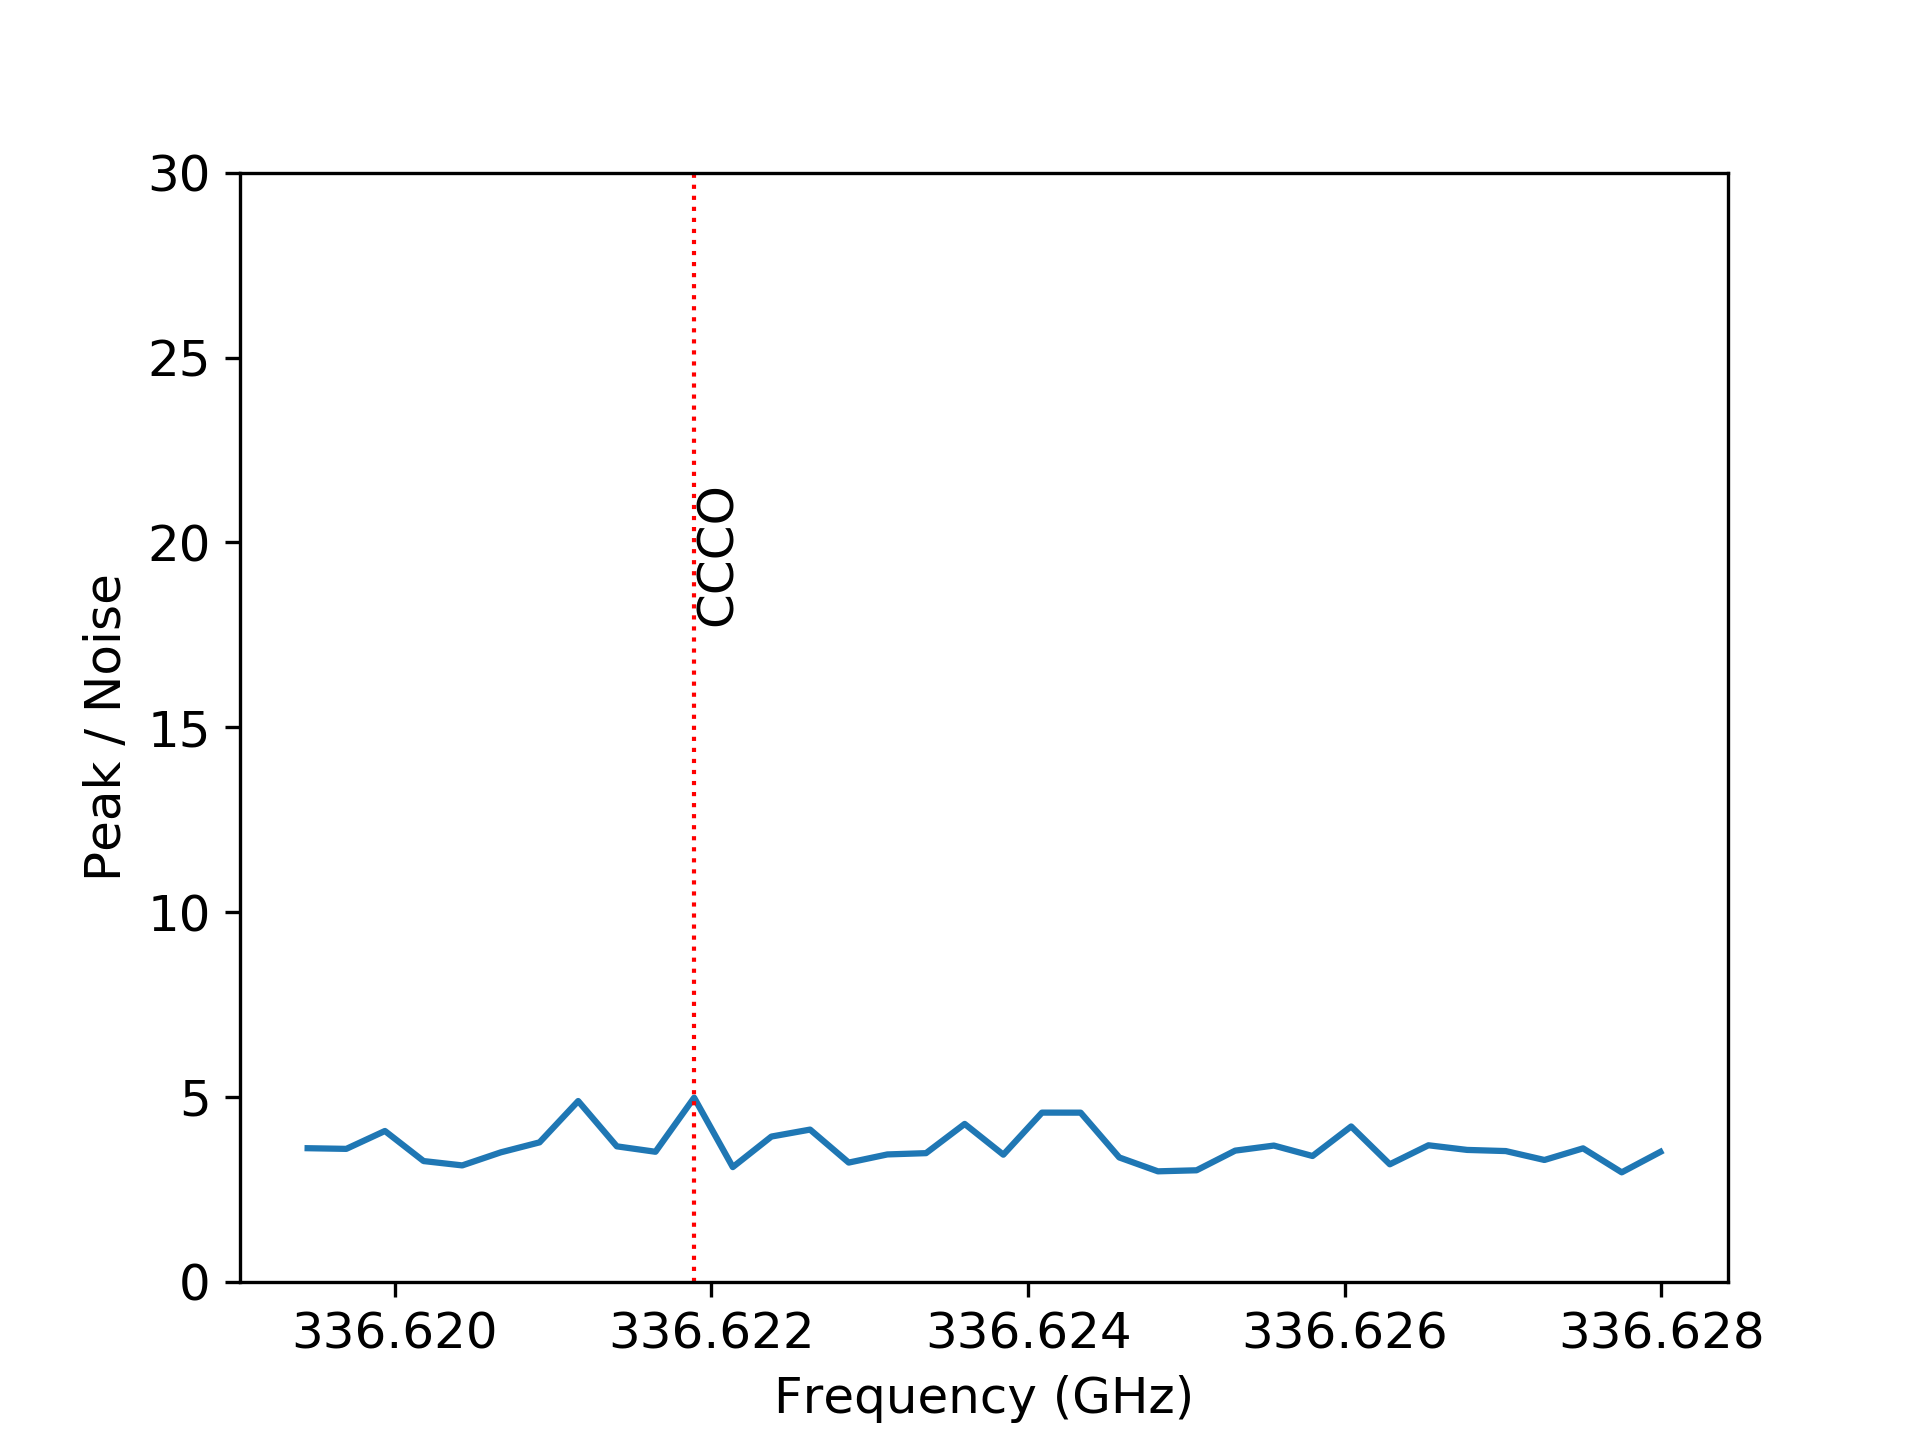
\includegraphics[width=0.33\textwidth]{spw1_CCCO}
    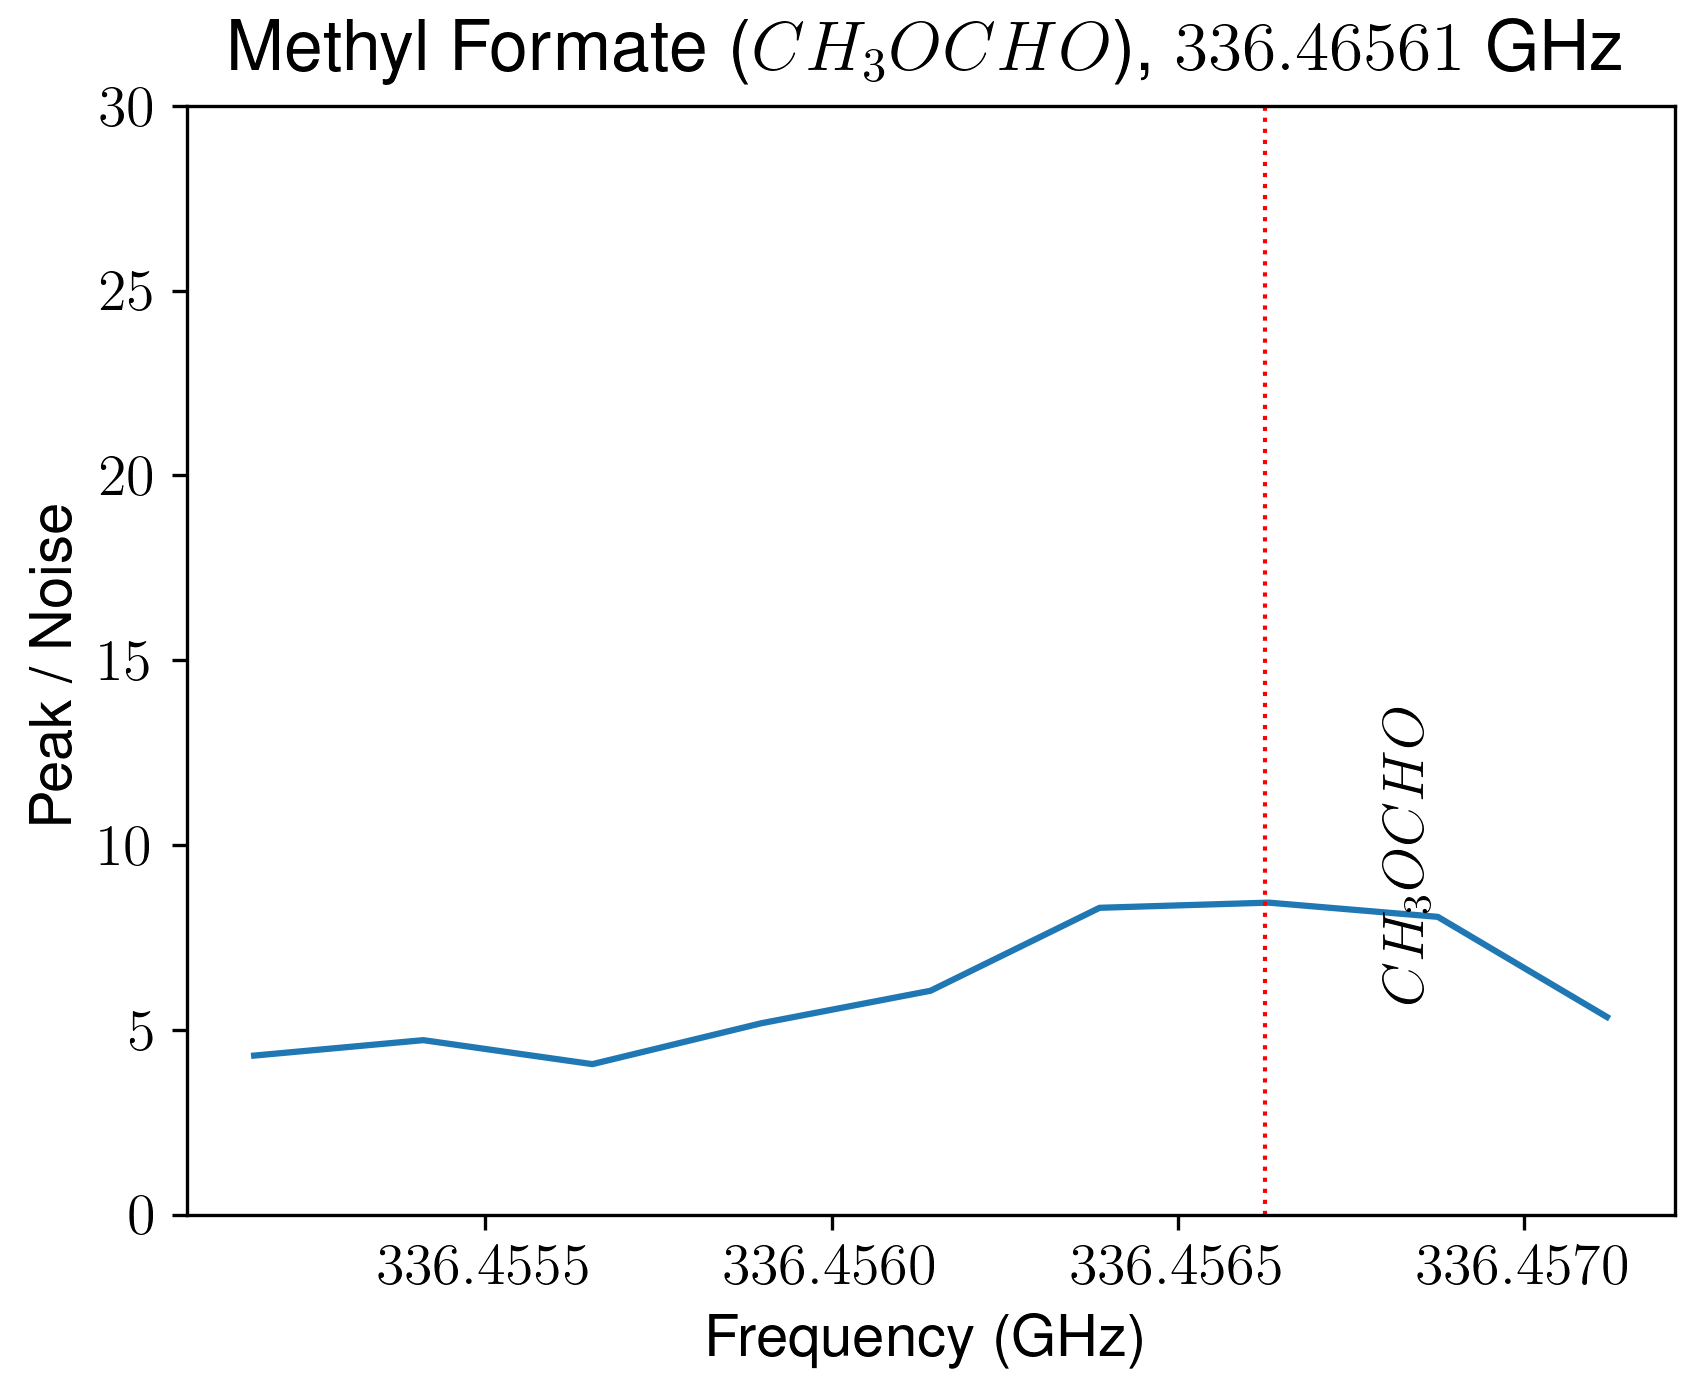
\includegraphics[width=0.33\textwidth]{spw1_CH3OCHO}
    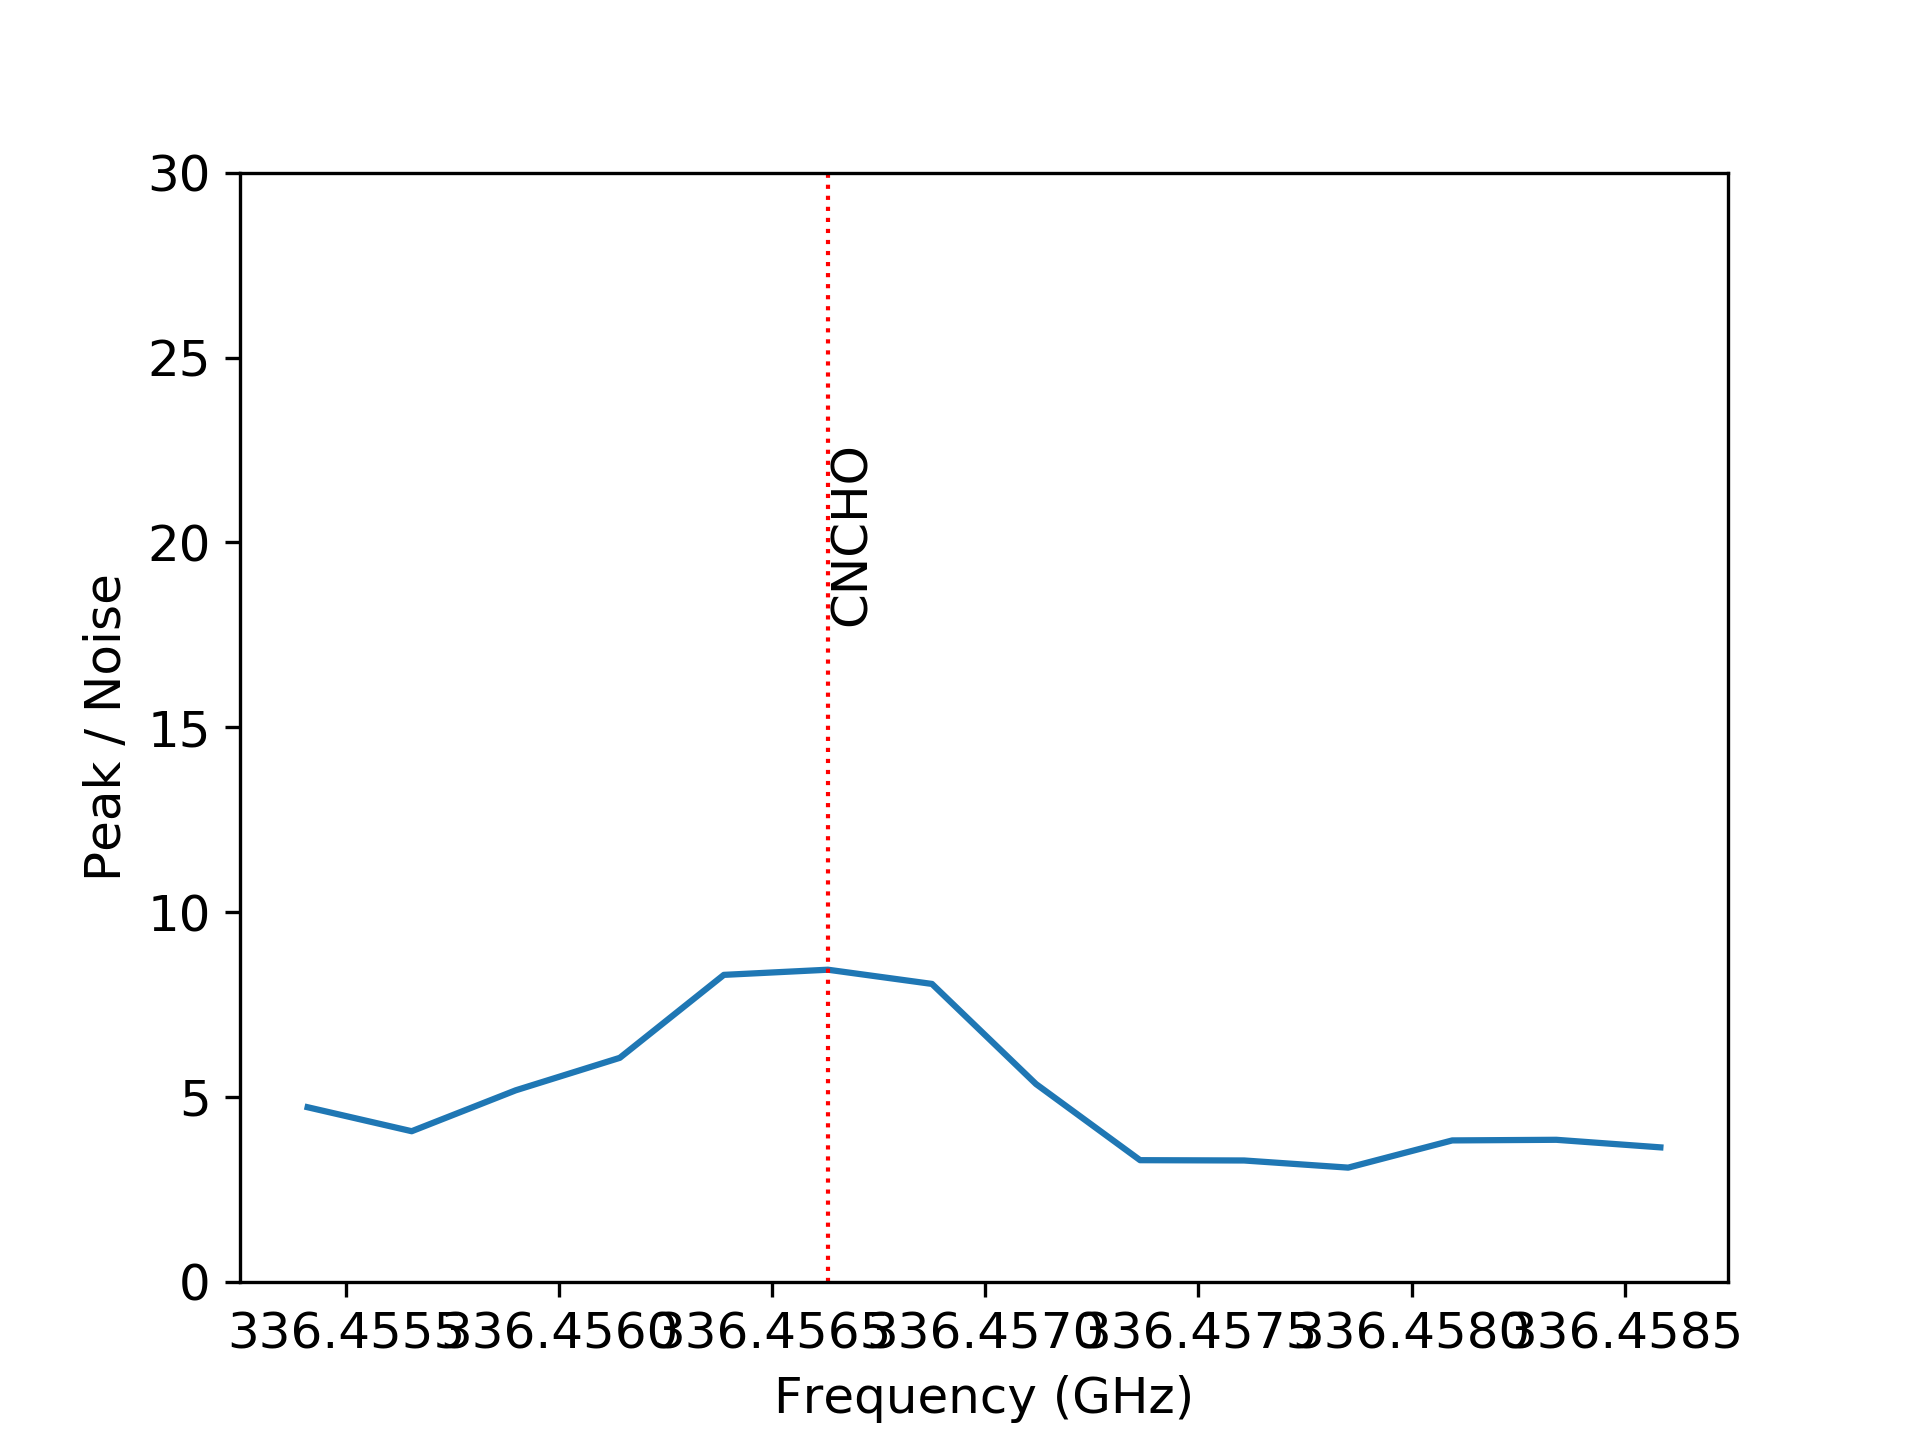
\includegraphics[width=0.33\textwidth]{spw1_CNCHO}
    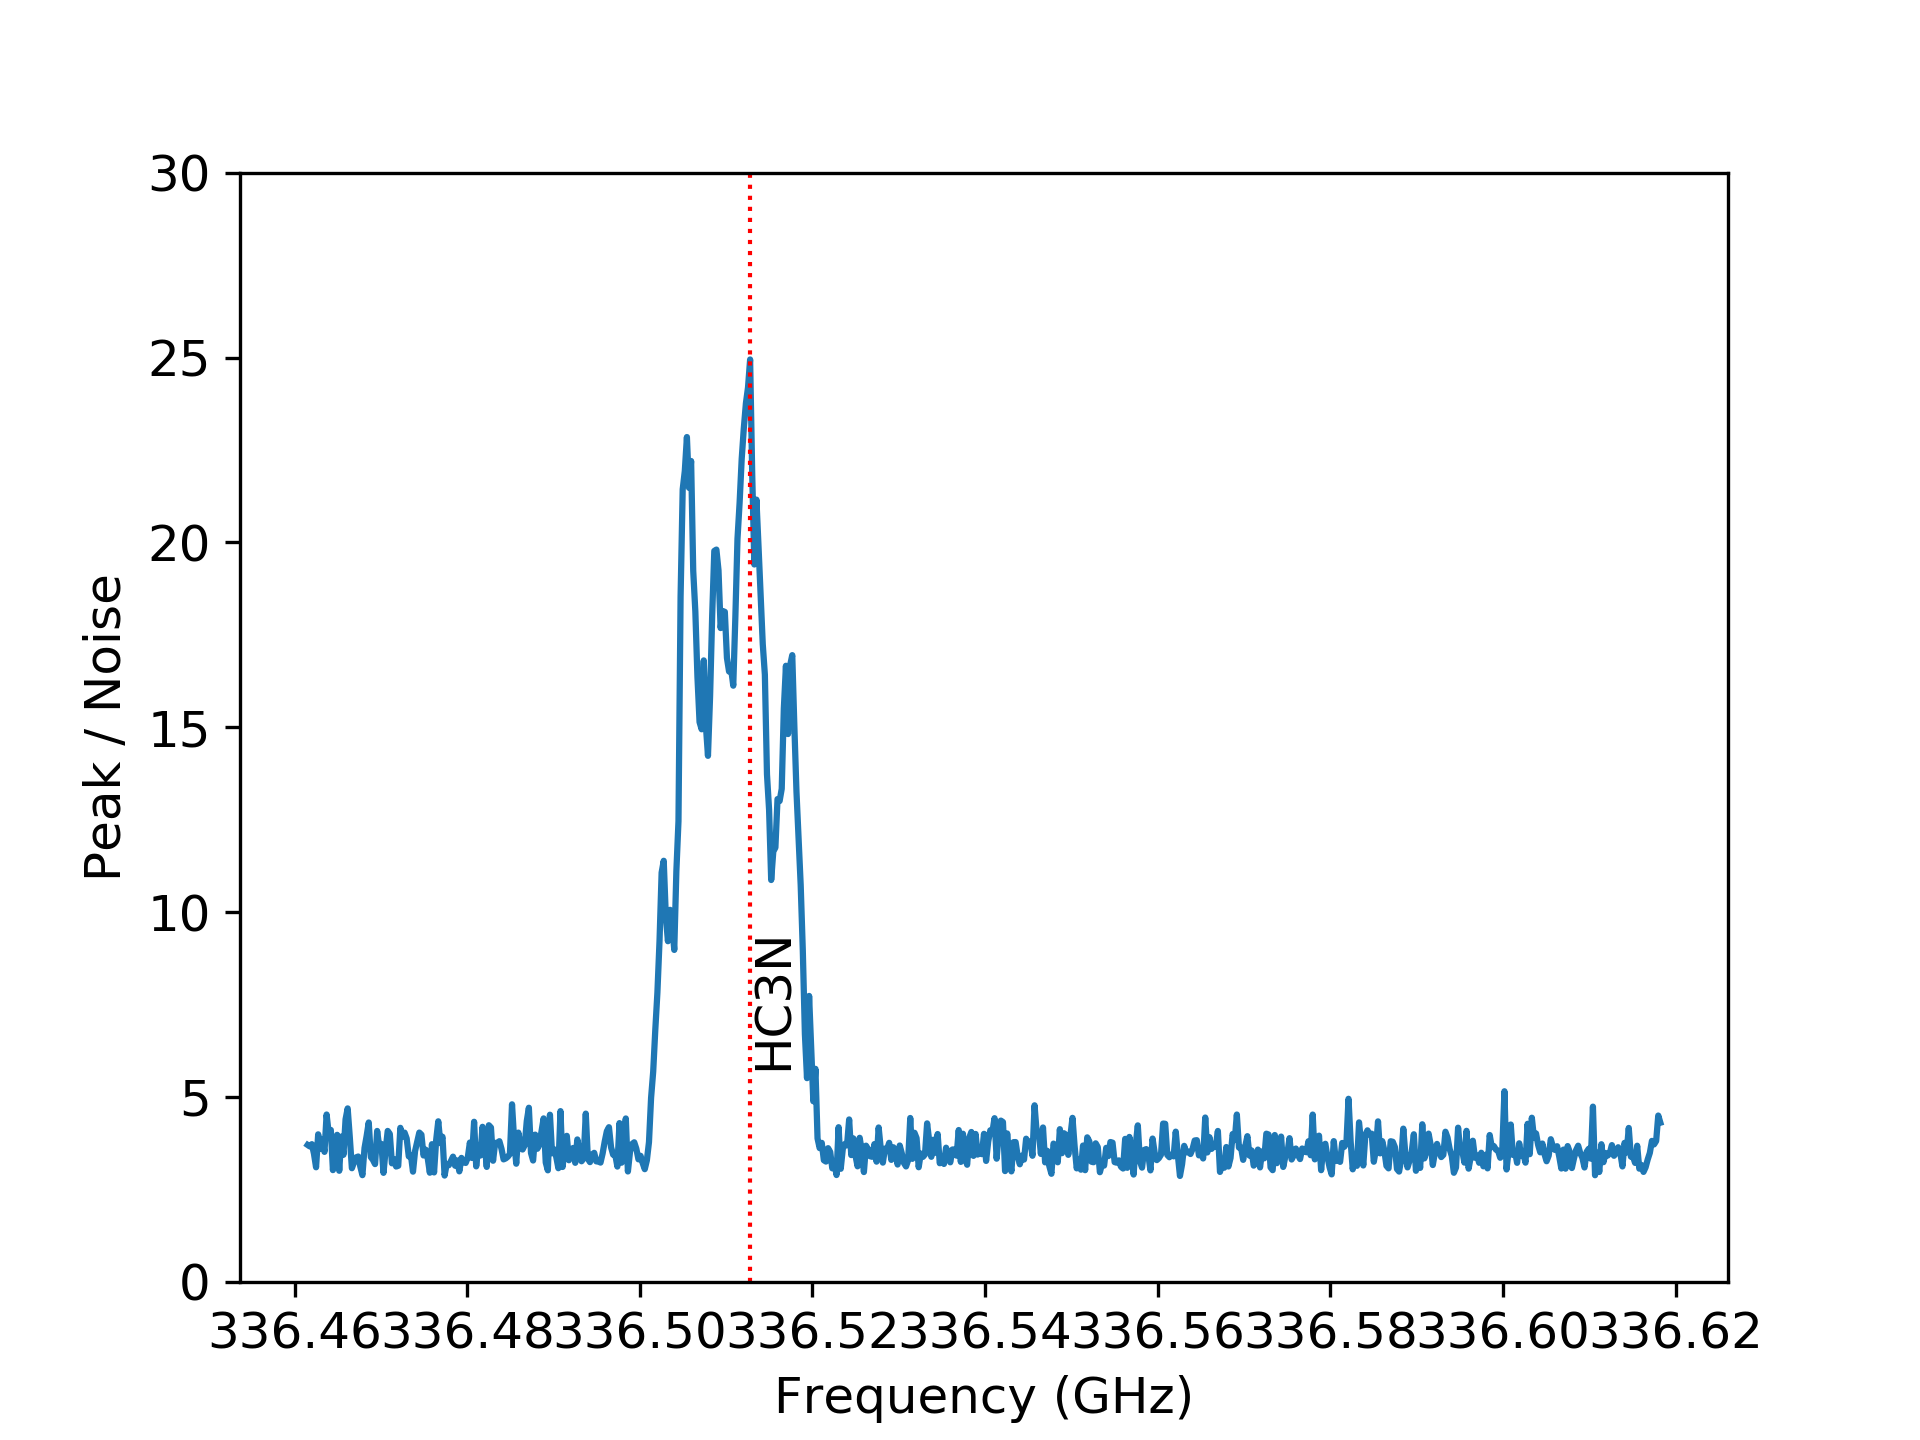
\includegraphics[width=0.33\textwidth]{spw1_HC3N}
    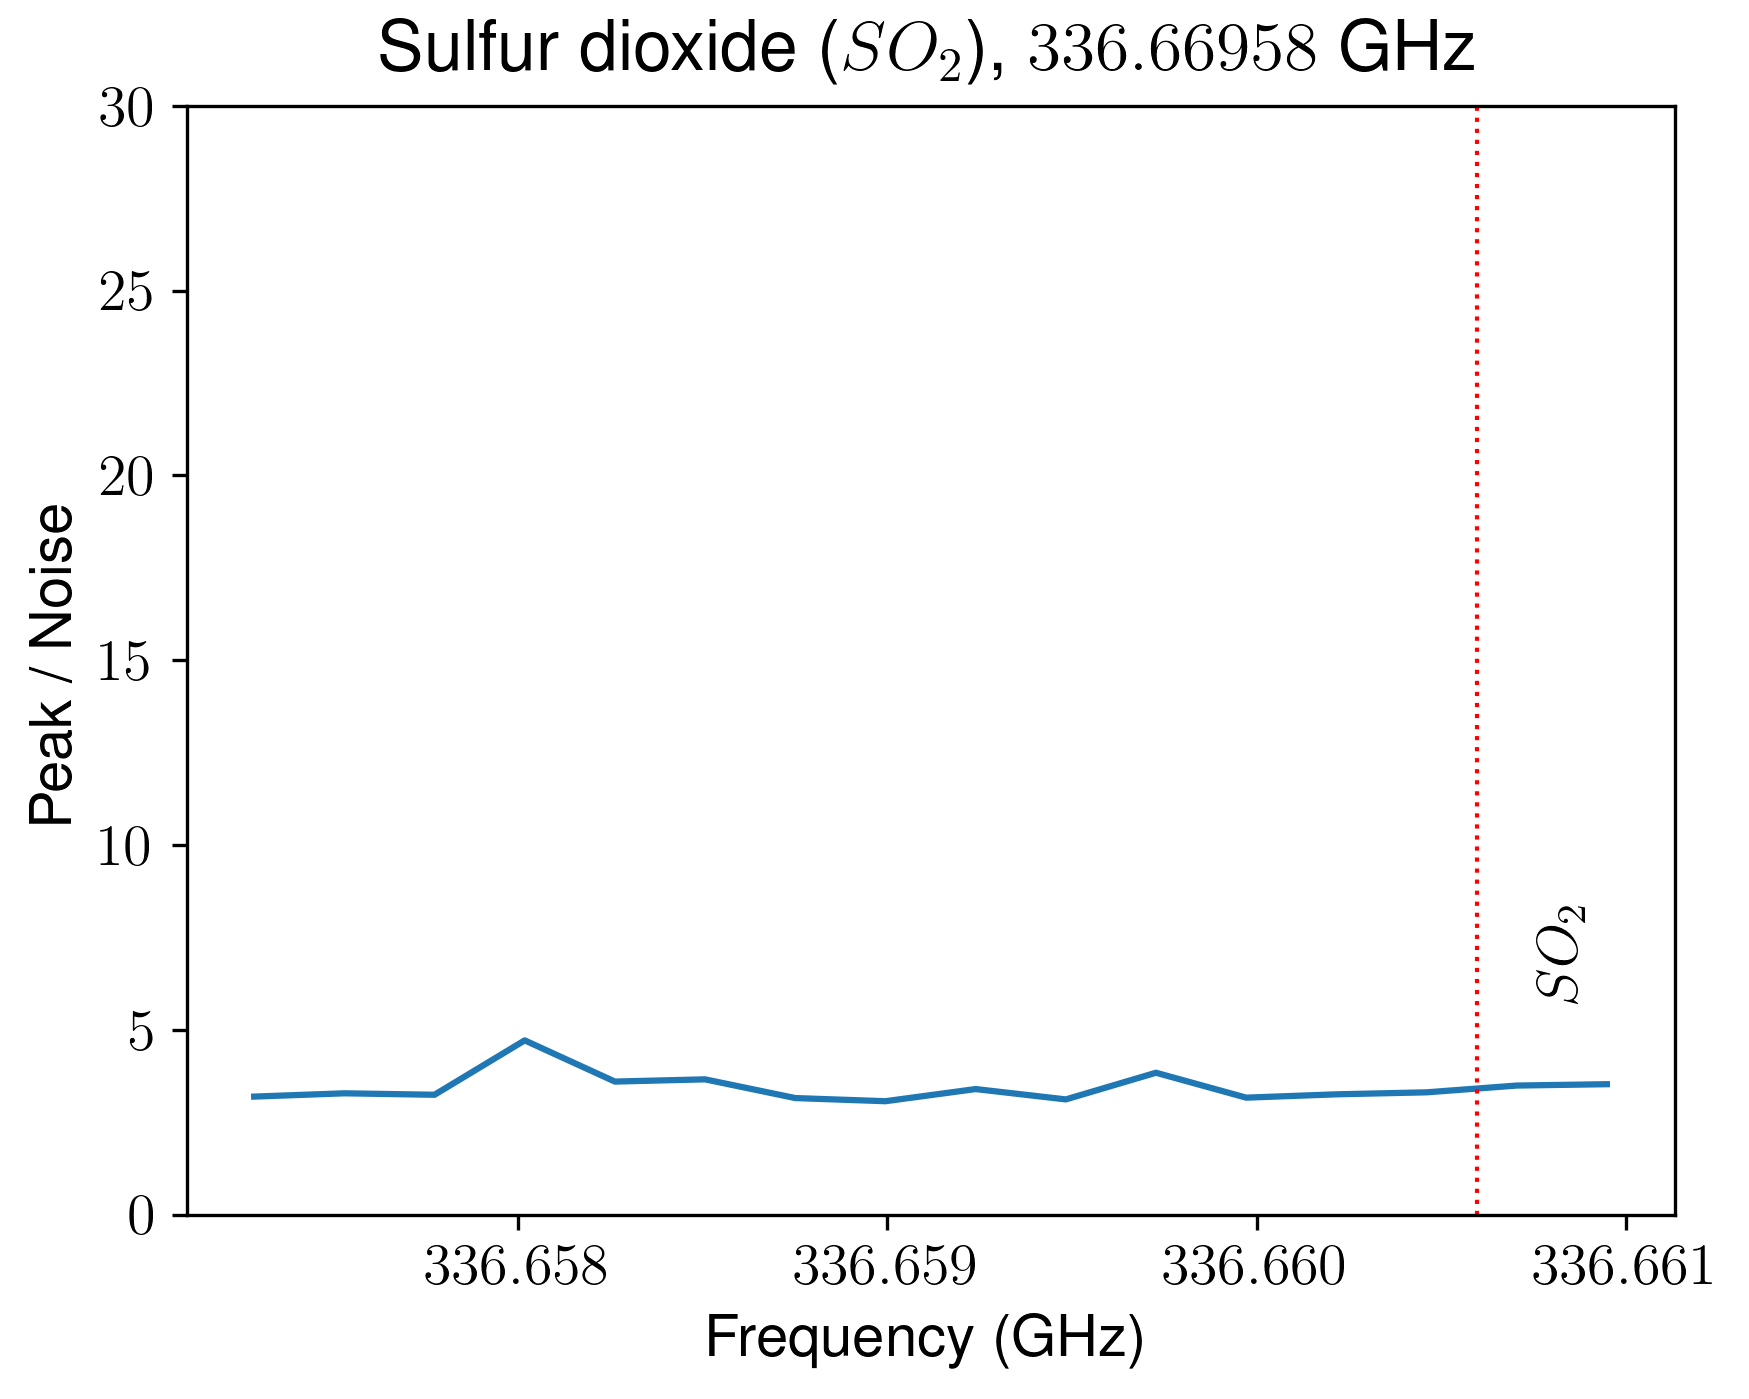
\includegraphics[width=0.33\textwidth]{spw1_SO2}
    \caption{Promising molecular lines identified in spectral window 1}
   \end{figure*}
   
\newpage 
   \begin{table}[htb]  
    \caption{\textbf{Line identification results for spectral window 2}}
    \tiny
    \centering    
    \begin{tabular}{l l l l l l l l l} 
    \hline     
    Molecule & Name &Transition & Frequency & $E_{u}$ & Intensity & Velocity & $v_{lsr}$ & Peak / rms\\ 
    \hline
$cis-CH_{2}OHCHO$ & Glycolaldehyde & $7_{6,2}-6_{4,3}$ & $334.05821$ & $37.4116$ & $45.0294$ & $6.5106$ & $8.0$ & $50.0827$\\
$CH_{3}OCHO$ & Methyl Formate & $15_{6,10}-14_{5,9}A$ & $334.10909$ & $94.8964$ & $17.0495$ & $9.9217$ & $8.0$ & $18.9629$\\
$CH_{3}NH_{2}$ & Methylamine & $17_{2}E1+1-17_{1}E1-1$ & $334.13094$ & $342.265$ & $10.4351$ & $14.8478$ & $8.0$ & $11.6061$\\
$_{33}SO_{2}$ & Sulfur Dioxide & $36_{11,25}-37_{10,28},F=69/2-71/2$ & $334.14626$ & $915.5991$ & $-0.6228$ & $8.9463$ & $8.0$ & $-1.4553$\\
$t-CH_{2}CHCHO$ & Propenal & $9_{3,7}-9_{1,8}$ & $334.20301$ & $37.7617$ & $3.1656$ & $6.2555$ & $8.0$ & $3.5209$\\
$CH_{3}NH_{2}$ & Methylamine & $8_{5}B1-9_{4}B2$ & $334.20979$ & $174.0493$ & $3.9923$ & $8.9327$ & $8.0$ & $4.4404$\\
$(CH_{3})_{2}CO$ & Acetone & $13_{11,3}-12_{8,4}AA$ & $334.21979$ & $80.4654$ & $-0.4388$ & $7.6194$ & $8.0$ & $-1.0253$\\
$CH_{3}OCHO$ & Methyl Formate & $29_{5,24}-28_{6,23}A$ & $334.23598$ & $282.1007$ & $3.9697$ & $1.2063$ & $8.0$ & $4.4152$\\
$_{13}CH_{3}OHvt=_{0}$ & Methanol & $3_{2,1}-2_{0,2}$ & $334.25221$ & $35.9468$ & $3.4457$ & $9.4204$ & $8.0$ & $3.8324$\\
$CP$ & Carbon Monophosphide & $N=7-6,J=15/2-13/2,F=8-7$ & $334.26182$ & $64.2111$ & $45.3174$ & $11.3104$ & $8.0$ & $50.4031$\\
$CH_{3}OCHO$ & Methyl Formate & $15_{6,9}-14_{5,9}E$ & $334.28144$ & $94.9147$ & $13.9904$ & $12.98$ & $8.0$ & $15.5604$\\
$g'Ga-(CH_{2}OH)_{2}$ & Ethylene Glycol & $15_{9,7}v=1-14_{8,7}v=0$ & $334.30955$ & $99.0907$ & $4.2402$ & $7.0359$ & $8.0$ & $4.7161$\\
$CH_{3}OHvt=_{1}$ & Methanol & $21_{5,16}-22_{4,19}$ & $334.32728$ & $964.3871$ & $6.4237$ & $12.1515$ & $8.0$ & $7.1446$\\
$s-H_{2}CCHOH$ & Vinyl Alcohol & $17_{4,13}-16_{4,12}$ & $334.34291$ & $182.2279$ & $15.4923$ & $6.892$ & $8.0$ & $17.2309$\\
$CH_{3}COOH$ & Acetic Acid & $30_{*,29}-29_{*,28}v=0$ & $334.37851$ & $259.444$ & $4.3631$ & $-4.0152$ & $8.0$ & $4.8527$\\
$g'Ga-(CH_{2}OH)_{2}$ & Ethylene Glycol & $24_{6,19}v=0-23_{5,18}v=0$ & $334.41275$ & $165.9969$ & $45.6615$ & $10.8101$ & $8.0$ & $50.7858$\\
$CH_{3}OHvt=_{1}$ & Methanol & $3_{0,3}-2_{1,2}$ & $334.42656$ & $314.4694$ & $52.4693$ & $7.1835$ & $8.0$ & $58.3575$\\
$g'Ga-(CH_{2}OH)_{2}$ & Ethylene Glycol & $13_{10,4}v=1-12_{9,4}v=0$ & $334.46125$ & $94.1713$ & $44.2048$ & $-2.9053$ & $8.0$ & $49.1656$\\
$(CH_{3})_{2}CO$ & Acetone & $13_{11,2}-12_{8,4}EE$ & $334.58973$ & $80.5543$ & $8.5715$ & $-10.7174$ & $8.0$ & $9.5334$\\
$t-CH_{3}CH_{2}OH$ & trans-Ethanol & $24_{7,17}-24_{6,18}$ & $334.60263$ & $313.8344$ & $12.3572$ & $5.1576$ & $8.0$ & $13.7439$\\
$CH_{3}OHvt=_{1}$ & Methanol & $22_{3,20}-22_{2,21}$ & $334.63249$ & $1001.3148$ & $13.0942$ & $11.6487$ & $8.0$ & $14.5637$\\
$CH_{3}OHvt=_{1}$ & Methanol & $25_{-3,22}-24_{-2,22}$ & $334.67771$ & $1073.8453$ & $21.2092$ & $-0.8691$ & $8.0$ & $23.5894$\\
$CH_{3}NH_{2}$ & Methylamine & $2_{2}A2-1_{1}A1,F=2-1$ & $334.71119$ & $22.5092$ & $0.0$ & $0.0$ & $8.0$ & $0.0$\\
$CCO$ & Oxoethenylidene & $N=14-13,J=14-14$ & $334.75876$ & $116.8058$ & $12.7521$ & $-3.4945$ & $8.0$ & $14.1832$\\
$(CH_{3})_{2}CO$ & Acetone & $12_{8,4}-11_{5,7}AE$ & $334.76545$ & $64.565$ & $20.6655$ & $11.5016$ & $8.0$ & $22.9846$\\
$CH_{3}CHO$ & Acetaldehyde & $17_{2,15}-16_{2,14}A++$ & $334.93139$ & $152.6118$ & $43.1424$ & $6.3067$ & $8.0$ & $47.9839$\\
$H_{213}CS$ & Thioformaldehyde & $10_{1,9}-9_{1,8}$ & $334.94932$ & $101.6033$ & $7.7273$ & $9.4859$ & $8.0$ & $8.5944$\\
$(CH_{3})_{2}CO$ & Acetone & $12_{8,4}-11_{5,7}EE$ & $334.99117$ & $64.4966$ & $13.4849$ & $-0.0038$ & $8.0$ & $14.9982$\\
$g'Ga-(CH_{2}OH)_{2}$ & Ethylene Glycol & $41_{17,24}v=0-41_{16,25}v=0$ & $335.07602$ & $565.0077$ & $0.462$ & $10.367$ & $8.0$ & $1.0795$\\
$c-H_{13}CCCH$ & Cyclopropenylidene & $5_{3,2}-5_{0,5}$ & $335.08781$ & $43.7198$ & $83.5866$ & $13.1283$ & $8.0$ & $92.9669$\\
$CH_{3}OHvt=_{0}$ & Methanol & $2_{2,1}-3_{1,2}--$ & $335.13369$ & $44.6721$ & $77.7538$ & $7.0251$ & $8.0$ & $86.4796$\\
$CH_{3}OCHO$ & Methyl Formate & $28_{4,24}-27_{5,23}A$ & $335.18332$ & $257.0799$ & $2.4819$ & $9.7965$ & $8.0$ & $2.7604$\\
$g-CH_{3}CH_{2}OH$ & gauche-Ethanol & $32_{6,27}-32_{5,27},vt=1-0$ & $335.2683$ & $545.844$ & $7.8166$ & $7.151$ & $8.0$ & $8.6938$\\
$CH_{3}CH_{2}CN$ & Ethyl Cyanide & $55_{8,48}-55_{7,49}$ & $335.27492$ & $733.8889$ & $7.8166$ & $8.2166$ & $8.0$ & $8.6938$\\
$HDO$ & Water & $3_{3,1}-4_{2,2}$ & $335.3955$ & $335.2672$ & $46.6299$ & $-58.3771$ & $8.0$ & $51.8628$\\
$HOCN$ & Cyanic acid & $16_{2,14}-15_{2,13}$ & $335.47103$ & $265.334$ & $3.6165$ & $14.814$ & $8.0$ & $4.0224$\\
$g-CH_{3}CH_{2}OH$ & gauche-Ethanol & $9_{4,5}-8_{3,6},vt=1-1$ & $335.48609$ & $118.6556$ & $39.5665$ & $1.356$ & $8.0$ & $44.0067$\\
$NHD_{2}$ & Ammonia & $1_{1,1}0s-0_{0,0}0s$ & $335.51385$ & $16.102$ & $47.0375$ & $68.9121$ & $8.0$ & $52.3161$\\
$CH_{3}OHvt=_{0}$ & Methanol & $7_{1,7}-6_{1,6}++$ & $335.58202$ & $78.9709$ & $56.2576$ & $-11.484$ & $8.0$ & $62.571$\\
$CH_{3}COOH$ & Acetic Acid & $15_{-15,0}-14_{-14,0}v=0$ & $335.60436$ & $128.6181$ & $10.8442$ & $-12.7636$ & $8.0$ & $12.0612$\\
$t-CH_{3}CH_{2}OH$ & trans-Ethanol & $23_{7,17}-23_{6,18}$ & $335.63059$ & $293.607$ & $17.1709$ & $8.6112$ & $8.0$ & $19.0979$\\
$cis-CH_{2}OHCHO$ & Glycolaldehyde & $21_{7,14}-21_{4,17}$ & $335.64676$ & $158.7973$ & $39.0976$ & $3.8067$ & $8.0$ & $43.4853$\\
$(CH_{3})_{2}CO$ & Acetone & $12_{11,1}-11_{8,4}EE$ & $335.67518$ & $71.4144$ & $24.4019$ & $8.8142$ & $8.0$ & $27.1404$\\
$cis-CH_{2}OHCHO$ & Glycolaldehyde & $68_{15,54}-68_{14,55}$ & $335.69367$ & $1456.6243$ & $-0.829$ & $8.4429$ & $8.0$ & $-1.9371$\\
$H_{2}NCH_{2}CN$ & Aminoacetonitrile & $21_{3,18}-20_{2,19}$ & $335.69558$ & $112.127$ & $-0.829$ & $6.7331$ & $8.0$ & $-1.9371$\\
$CH_{3}OHvt=_{0}$ & Methanol & $25_{8,17}-26_{7,20}++$ & $335.7015$ & $1073.9686$ & $0.0$ & $0.0$ & $8.0$ & $0.0$\\
$t-H_{13}COOH$ & Formic Acid & $6_{3,3}-7_{1,6}$ & $335.71489$ & $50.4224$ & $13.3501$ & $-0.5284$ & $8.0$ & $14.8482$\\
$CH_{3}NH_{2}$ & Methylamine & $14_{1}E1-1-13_{2}E1-1$ & $335.74509$ & $225.3446$ & $12.4894$ & $4.6287$ & $8.0$ & $13.8909$\\
$CH_{3}COOH$ & Acetic Acid & $13_{11,2}-12_{9,3}--v=0$ & $335.77985$ & $89.7941$ & $15.7797$ & $3.9964$ & $8.0$ & $17.5506$\\
$(CH_{3})_{2}CO$ & Acetone & $32_{2,30}-31_{3,29}EA$ & $335.80289$ & $281.4994$ & $0.0$ & $0.0$ & $8.0$ & $0.0$\\
$(CH_{3})_{2}CO$ & Acetone & $32_{2,30}-31_{2,29}AE$ & $335.80291$ & $281.4994$ & $11.5028$ & $1.213$ & $8.0$ & $12.7937$\\
$H_{2}C_{18}O$ & Formaldehyde & $5_{1,5}-4_{1,4}$ & $335.81594$ & $60.2335$ & $31.1124$ & $7.7668$ & $8.0$ & $34.6039$\\
$CH_{3}CH_{2}CN$ & Ethyl Cyanide & $10_{4,6}-10_{1,9}$ & $335.84026$ & $41.4386$ & $16.3359$ & $3.3581$ & $8.0$ & $18.1692$\\
$CH_{3}OCHO$ & Methyl Formate & $27_{9,19}-26_{9,17}E$ & $335.89969$ & $277.8455$ & $4.5668$ & $11.5288$ & $8.0$ & $5.0793$\\
    \hline                  
    \end{tabular}
\end{table}





\end{document}
